\documentclass{diploma}

\student{Инютин Максим Андреевич}
\group{М8О-407Б-19}
\theme{Создание модуля управления временными рядами сигналов для системы активного мониторинга сложных технических систем}

\supervisor{Дзюба Дмитрий Владимирович}
\firstConsultant{---}
\secondConsultant{---}
\reviewer{---}

\faculty{№ 8 <<Компьютерные науки и прикладная математика>>}
\department{806}
\speciality{01.02.03 <<Прикладная математика и информатика>>}
\profile{Информатика}

% Здесь необходим разрыв строки из-за особенностей титульной страницы
\departmentFullName{№ 806}
\headOfDepartment{Крылов Сергей Сергеевич}

% Дата. Оставляем пустое место для дня
\date{\uline{\hspace{24pt}} мая \the\year\ года}

\newglossaryentry{bd}{
    name={База данных},
    description={набор информации, которая хранится упорядоченно в электронном виде}
}

\newglossaryentry{time-series}{
    name={Временной ряд},
    description={собранный в разные моменты времени статистический материал о значении каких-либо параметров исследуемого процесса}
}

\newglossaryentry{tree}{
    name={Дерево},
    description={связный ациклический граф}
}

\newglossaryentry{freq}{
    name={Частота дискретизации},
    description={частота взятия отсчётов непрерывного по времени сигнала при его дискретизации}
}

\newacronym{db}{БД}{база данных}

\newacronym{dbms}{СУБД}{система управления базами данных}


\addbibresource{main.bib}

% Иллюстрации всегда по центру
\makeatletter
\g@addto@macro\@floatboxreset\centering
\makeatother
    
\begin{document}
\maketitle

% \includepdf[pages=-]{extra/task} % Задание
\setcounter{page}{2} % Устанавливает счётчик страниц

\abstract % Структурный элемент: РЕФЕРАТ

\keywords{ЦИФРОВОЙ ДВОЙНИК, РЕЛЯЦИОННЫЕ БАЗЫ ДАННЫХ, ВРЕМЕННЫЕ РЯДЫ, СОРТИРОВКА, ДВА УКАЗАТЕЛЯ, ДЕРЕВЬЯ, ПОИСК В ГЛУБИНУ}

Объектом разработки в данной работе является часть цифрового двойника электростанции.

Цель работы --- является разработать модуль, обеспечивающий управление структурой хранения временных рядов и данными сенсоров для системы мониторинга цифрового двойника промышленных электростанций, использующих газотурбинное оборудование.

Основное содержание работы состояло в разработке алгоритма управления графом организационной структурой и объединения данных датчиков с разными частотами дискретизации.

Основным результатом работы является модуль управления временными рядами сигналов сложных технических систем на языке Python с использованием СУБД PostgreSQL и ClickHouse.

Данные результаты разработки предназначены для надёжного хранения данных датчиков и последующего использования при моделировании объекта и предиктивной аналитики.

Внедрение модуля позволяет автоматизировать сбор информации с сенсоров системы, тем самым упрощая создание цифрового двойника электростанции.
 % Реферат

\tableofcontents % Содержание 
\termsanddefenitions % Термины и определения
\listofabbreviations % Перечень сокращений и обозначений

\introduction % Структурный элемент: ВВЕДЕНИЕ

Актуальность темы данной работы связана с распространением цифровых двойников объектов и систем. Их создание позволяет моделировать отдельные процессы или объекты целиком, проводить тесты, анализировать полученные данные для подбора оптимальных параметров системы. Один из способов создания цифрового двойника — установка сенсоров и сбор данных с них. Полученную информацию необходимо систематизировать и хранить. На предприятии может быть очень много оборудования, поэтому нужно внедрять эффективный и надёжный модуль хранения данных датчиков.

Таким образом, выполненная работа актуальна и с теоретической, и с практической точек зрения.

Цель работы --- разработать модуль, обеспечивающий управление структурой хранения временных рядов и данными сенсоров. Для достижения поставленной цели в работе были решены следующие задачи:

\begin{itemize}
    \item спроектирована модель данных дерева организационной структуры предприятия;
    \item описаны способы взаимодействия: добавление, удаление и изменение вершин и рёбер дерева;
    \item спроектирована модель хранения временных рядов датчиков;
    \item изучены средства и технологии, которые будут применятся в ходе разработки программного продукта;
    \item реализован модуль управления графом организационной структурой и данными;
    \item разработан алгоритм объединения данных датчиков с разными частотами дискретизации;
    \item реализована генерация данных для таблиц датчиков, алгоритм получения наборов временных рядов;
    \item произведён тест производительности реализованного модуля, проведено сравнение двух алгоритмов хранения и считывания данных.
\end{itemize}

Для разбработки программы необходимо изучить инструменты и методы, решающие поставленные задачи. Работа основывается на следующих СУБД, библиотеках, технологиях и алгоритмах:

\begin{itemize}
    \item Python является основным языком программирования, который использовался при решении задач;
    \item FastAPI реализует веб-интерфейс для взаимодействия с модулем и базами данных, SwaggerUI визуализирует веб-интерфейс;
    \item SQLAlchemy позволяет работать с базами данных на основе объектно-ориентированного подхода;
    \item PostgreSQL обеспечивает хранение дерева организационной структуры предприятия и информации о датчиках;
    \item ClickHouse хранит большие объёмы данных, получаемые от сенсоров;
    \item Docker позволяет разворачивать и переносить изолированные контейнеры с базами данных;
    \item GraphViz визуализирует дерево организационной структуры;
    \item метод двух указателей используется для объединения таблиц датчиков с разными частотами дискретизации.
\end{itemize}

В результате выполнения работы был разработан модуль управления временными рядами и деревом организационной структуры предприятия, позволяющий генерировать и полученать наборы временных рядов, управлять, изменять, визуализировать граф организационной структуры, добавлять новые датчики и организационные единицы.

Результаты работы предназначены для автоматизации сбора данных данных с датчиков, установленных на предприятии. Собранные данные передаются в базу данных для последующего мониторинга, диагностики и аналитики, расчёта оптимальных параметров на предприятии.

Использование разработки позволяет ускорить процесс создания цифрового двойника системы, а так же сделать его более точным. Модуль обеспечивает надёжное хранение организационной структуры предприятия и быстрый доступ к данным сенсоров оборудования. % Введение

\section{ЦИФРОВЫЕ ДВОЙНИКИ КОМПАНИИ}

\subsection{Цифровые двойники, их применение и автоматизация создания}

Цифровой двойник --- это виртуальная копия объекта или системы, созданная на основе данных, полученных из реального мира. Цифровые двойники могут быть созданы для любого объекта или системы, от автомобилей до зданий и даже городов.

Они используются в различных сферах и областях, включая проектирование и строительство, управление городами и транспортом, энергетику и промышленность, медицину и многое другое. Цифровые двойники позволяют смоделировать объект или систему в виртуальной среде, чтобы оптимизировать его производительность, улучшить безопасность и снизить затраты.

Одним из наиболее распространенных применений цифровых двойников является проектирование и строительство зданий. Цифровые двойники зданий могут использоваться для оптимизации проектирования, улучшения эффективности энергопотребления и сокращения времени строительства. В промышленности цифровые двойники используются для оптимизации производственных процессов, улучшения качества продукции и снижения затрат на производство. Цифровые двойники могут помочь смоделировать производственную линию и определить оптимальные настройки оборудования для снижения изонса. Они также используются в медицине для создания виртуальных моделей пациентов. Это позволяет врачам более точно диагностировать и лечить заболевания, а также планировать сложные операции.

В целом, цифровые двойники становятся все более распространенными и играют важную роль в различных областях. Они помогают улучшить безопасность и экономическую эффективность объектов и систем, а также ускоряют процесс разработки и производства.

Для автоматизации создания цифровых двойников необходимы компьютерные алгоритмы и технологии, создающие копии объектов и систем. Такой подход позволяет не только ускорить процесс создания цифровых двойников, но и улучшить их точность и качество.

Одним из распространенных методов автоматизации создания цифровых двойников является использование программного обеспечения для моделирования. Это позволяет создавать точные виртуальные модели объектов и систем на основе данных, полученных из реального мира. Программное обеспечение может быть настроено для определения оптимальных параметров объекта или системы, а также для проведения различных симуляций и тестов.

Ещё одним методом является использование искусственного интеллекта и машинного обучения. Это позволяет создавать более точные и детальные модели объектов и систем, а также оптимизировать процесс создания цифровых двойников. Искусственный интеллект может быть настроен для обработки больших объемов данных и автоматического анализа полученной информации.

Автоматизация создания цифровых двойников имеет большое значение для различных отраслей энергетики, промышленности, медицины, строительства и других областей. Не менее важно собирать и хранить данные объекта для создания цифрового двойника.

Автоматизировать сбор данных с объекта можно с помощью различных сенсоров, таких как лазерные сканеры, фотокамеры, акселерометры, гироскопы и другие. Датчики могут быть установлены на объекте или системе и использоваться для удалённого сбора данных. Собранные данные затем обрабатываются и хранятся в базе данных.

Другим методом автоматизации сбора данных является использование систем мониторинга и диагностики. Эти системы могут быть установлены на объекте или системе и использоваться для непрерывного мониторинга и анализа различных параметров, таких как температура, давление, вибрация, электрические параметры и другие. Собранные данные затем передаются в базу данных для дальнейшей обработки и хранения.

Поступающих данных может быть очень много, поэтому важно быстро и эффективно сохранять их в базе данных. Потери этих данных недопустимы, так как могут привести к серьёзным последствиям при моделировании объекта или системы, для которой создаётся цифровой двойник.

\subsection{Этапы, результаты и сложности при создания цифровых двойников предприятия}

С ростом цифровизации в различных отраслях растёт и развитие цифровых двойников в промышленности и энергетике. По данным~\cite{Habr1} на 2021 год 18 ведущих мировых компаний уже используют цифровые двойники, а 24 тестируют их применение. В России к 2024 250 ведущих компаний планируют внедрить эту технологию.

Создание цифровых двойников --- достаточно сложный процесс, который можно разделить на следующие этапы~\cite{Habr2}:

\begin{itemize}
    \item обследование начинается с изучения нормативных документов, карт и инструкций по экплуатации, часто информация не закреплена или исполнятся не строго по бумагам, поэтому необходимо проводить интервью с работниками для воспроизведения процессов на предприятии максимально близким к реальным;
    \item разработка обычно является самым долгим и трудным этапом, необходимо создать инфраструктуру предприятия в виртуальной среде, разбработать программные продукты для взаимодействия;
    \item валидация заключается в проверке точности модели на основе данных работы предприятия в прошлом, чем ниже расхождение модели с реальной работой, тем выше качество модели;
    \item эксплуатация --- цифровой двойник внедряется в работу и используется для решений актуальных задач предприятия.
\end{itemize}

В зависимости от степени цифровизации предприятия срок создания цифрового двойника варьируется от трёх месяцев до года. Чем выше готовность бизнеса к цифровизации, тем проще проходят описанные выше этапы. Рассмотрим несколько примеров из~\cite{Habr1}, как цифровые двойники улучшили работу на предприятиях.

Морской порт на юге России нуждался в оптимизации распределения нагрузки и планирования смен. Все данные передавались на бумаге, их вручную обрабатывал оператор. Такой подход сильно зависит от человеческого фактора --- вероятность ошибки и скорость работы зависит от оператора. Создание цифрового двойника позволило лучше составлять планы, что повысило среднесуточные объёмы перевалки на $4\%$, а как следствие и выручку порта.

Одна из ведущих горнодобывающих групп в СНГ на одном из принадлежащих ей угольных карьеров часто не выполняла планы по извлечению вскрышки, это приводило к срыву планов по добыче угля. Одно из проблемных мест --- нормативные данные по длительности операций устарели и не соответствовали реальным. Для создания модели карьера длительность всех операций замерялась секундомером. Благодаря точному моделированию работы угольный шахты в виртуальной среде стало возможным оценить потенциал наращивания производственных мощностей и свести к минимуму простой оборудования и техники из-за отсутсвия запчастей.

\subsection{Техническое задание}

Как было описано выше, одна из задач для создания цифрового двойника --- сбор и хранение данных, собираемых с системы. Необходиму решить эту задачу для последующего создания полноценного цифрового двойника и применения алгоритмов моделирования и машинного обучения.

Для работы системы мониторинга и предиктивных моделей с объектов предприятия собираются исходные данные. Оборудование оснащено датчиками, собирающими данные с разными частотами дискретезации.

Так как оборудование взаимосвязано и образует сложные технологические цепочки, границы принадлежности датчика к тому или иному оборудованию размыты. Один датчик может входить в состав моделей для разных единиц оборудования. Однако все датчики могут быть однозначно отнесены к одному объекту организационной структуры предприятия. Количество всех параметров для одного объекта может составлять несколько тысяч.

Задачей является разработать модуль, обеспечивающий управление структурой хранения временных рядов и данными сенсоров для системы мониторинга цифрового двойника промышленных электростанций, использующих газотурбинное оборудование. Временные ряды должны хранится в ClickHouse, а справочники в PostgreSQL. При реализации необходимо предусмотреть следующие особенности:

\begin{itemize}
    \item возможность определять структуру таблиц --- наборы и типы датчиков к привязке к оргнизационной структуре;
    \item частота дискретезации датчиков может быть разной: в какой-то момент времени не у всех датчиков есть значение, тогда это событие достраивается по последнему известному значению на этот момент;
    \item датчики имеют глобальные уникальные идентификаторы;
    \item для получения данных должна быть возможность получать вектора (все значения датчиков), временной ряд, набор рядов;
    \item механизм настройки, который будет позволять сопоставлять код датчика к организационной единице;
    \item дерево оборудования связано с сигналами отношением многие ко многим.
\end{itemize} % Глава 1
\section{РАЗРАБОТКА ПРОГРАММНОГО ПРОДУКТА}

\subsection{Модель организационной структуры и сенсоров, способы взаимодействия с данными}

Организационная структура предприятия представима в виде дерева. Поэтому можно хранить дерево как неориентированный граф~\cite{graphs}, что позволит легко добавлять новые организационные единицы и сенсоры, создавать и удалять связи между ними. На рисунке~\ref{datamodel} показана модель графа организационный структуры. Типы данных соответствуют типам СУБД PostgreSQL~\cite{pg-datatypes}.

\begin{figure}
  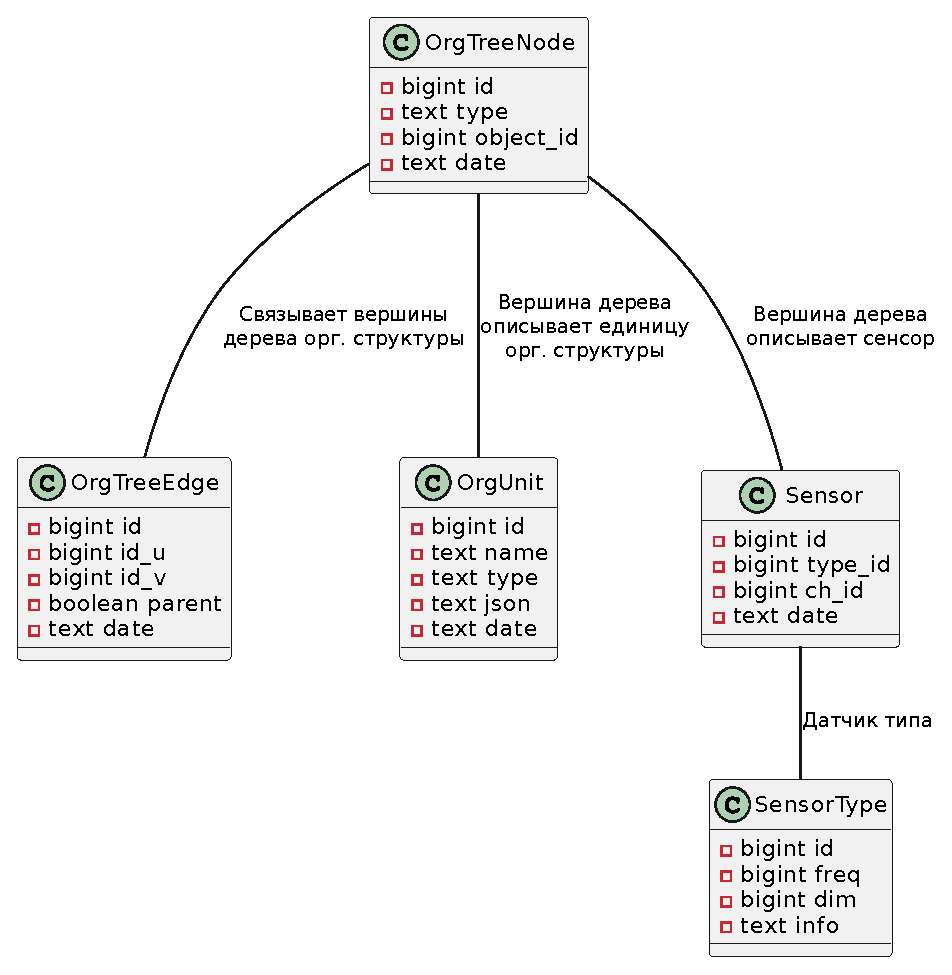
\includegraphics[scale=1.0]{../img/datamodel.eps}
  \caption{Модель организационной структуры}
  \label{datamodel}
\end{figure}

Основные способы управления временными рядами и деревом организационной структуры приведены на рисунке~\ref{usecases}.

\begin{figure}
  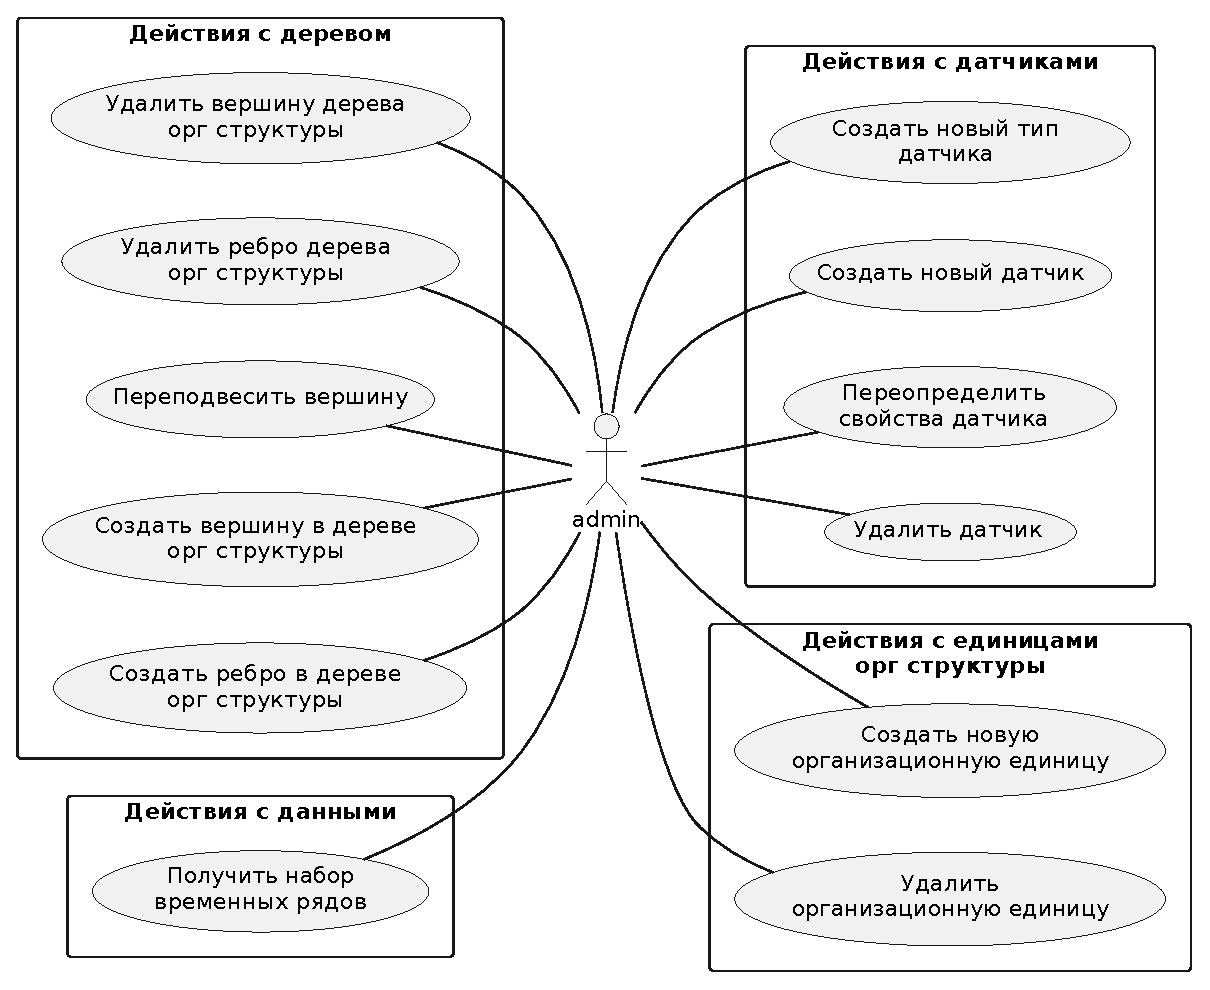
\includegraphics[scale=0.8]{../img/usecases.eps}
  \caption{Способы взаимодействия}
  \label{usecases}
\end{figure}

OrgTreeNode --- вершина графа организацонной структуры. Хранит уникальный идентификатор вершины, тип объекта (сенсор или единица организационной структуры) и его номер.

OrgTreeEdge --- ребро графа организационной структуры. id\_u и id\_v хранят начальную и конечную вершины ребра. parent указывает, является ли ребро от родителя к рёбенку или нет.  Уникальный идентификатор id нужен для реализации получения обратного ребра.

OrgUnit описывает единицу организационной структуры, имеет свой уникальный идентификатор. Поля name, type, json используются для хранения информации об единице и могут быть изменены при необходимости.

SensorType описывает тип датчика --- его частоту дискретизации и размерность данных, которые регистрирует датчик. info хранит служебную информацию о типе. Уникальный идентификатор id используется, чтобы задать тип определённому сенсору.

Sensor описывает датчик, так же имеет свой уникальный идентификатор. type\_id хранит идентификатор типа датчика, описанный выше. ch\_id содержит номер таблицы, в которой хранятся данные, регистрируемые датчиком.

Поля date обозначают, когда был удалён объект организационной структуры. Если объект не удалён, оно будет пустым. Это поле позволяет реализовать историю всех объектов организационной структуры, добавляя к модели персистентность.

Чтобы создать новый сенсор, нужно узнать, добавлен ли тип сенсора, затем добавить новый сенсор, создав под него новую таблицу. Добавление новой организационной единицы не требует никаких проверок.

Для создания вершнины дерева требуется определить, будет ли вершина соответствовать организационной еденице или датчику. Затем проверить, что соответствующая единица или датчик существуют на момент создания вершины.

При создании ребра между двумя вершинам выполняется проверка, что такое ребро не существует, чтобы избежать добавления кратных рёбер. Так же проверяем, что ребро не является петлёй. Добавляем два ребра --- прямое ребро $(u, v)$ с номером $id$ и истинным флагом $parent$, обратное $(v, u)$ с номером $id + 1$. Такое хранение рёбер позволяет получать обратное ребро. Допустим, без потери общности, индексация рёбер начинается с нуля. Если это не так, то при вычислении вычтем единицу. Пусть ребро $(u, v)$ имеет идентификатор $id$, тогда обратное ему ребро --- $id - 1$ либо $id + 1$. Если $(u, v)$ --- прямое ребро, то $id$ чётное или ноль, обратное ему --- $id + 1$, что так же равно $id \oplus 1$. Если $(u, v)$ --- обратное ребро, то $id$ нечётное, обратное ребро имеет номер $id - 1$, что опять же равно $id \oplus 1$, так как младший бит в $id$ равен единице, после применения операции побитового исключающего ИЛИ~\cite{XOR} с единицей станет нулём. Таким образом для получения обратного ребра необходимо выполнить побитовое исключающее ИЛИ номера ребра с единицей.

Удаление единицы организационной структуры или датчика осуществляется изменением поля $date$ на сегодня. Для удаления ребра найдём номер ребра и пометим его сегодняшней датой. То же самое сделаем и для обратного ребра, которое получим по принципу, описанному выше.

Для удаления вершины $u$ найдём её номер и номер ребра в родителя, пометим их сегодняшним числом. Теперь нужно каскадно удалить всё поддерево с корнем в этой вершине. Сформируем список смежности~\cite{graphs} вершины, используя таблицу с рёбрами дерева. Необходимо удалять только детей вершины $u$, поэтому выбираем рёбра с истинным флагом $parent$. Выполним обход в глубину~\cite{dfs1, dfs2} из вершины $u$ по этим рёбрам, вызывая функцию удаления. Обход в глубину имеет сложность $O(n + m)$, где $n$ --- количество вершин в поддереве, $m$ --- количество рёбер. Так как корневое поддерево~\cite{rooted-trees} сохраняет свойства дерева, $m = n - 1$, поэтому сложность $O(n)$.

Для переподвешивания вершины нужно сперва удалить ребро, соединяющее её с родителем, а затем добавить новое ребро.

Для визуализации дерева организационной структуры в реальном времени достаточно выбрать всё содержание таблиц, содержащих вершины и рёбра дерева. Удалённые элементы помечены какой-то датой, для выборки объектов, существующий на данных момент времени, следует выбирать записи, в которых поле $date$ пустое.

С помощью обхода в глубину так же осуществляется сбор данных с датчиков, находящихся в поддереве организационной единицы. Обход находит все таблицы датчиков и необходимые столбцы, после чего происходит выборка и интерполяция значений датчиков. Подробно объединение значений датчиков описано ниже.

\subsection{Стек используемых технологий}

Программный продукт реализован на языке программирования Python~\cite{Python}. Он имеет простой и понятный синтаксис. Динамическая типизация обеспечивает высокую скорость разработки. Большой набор стандартных библиотек позволяет решать широкий спекрт задач. С помощью встроенного менеджера пакетов pip возможно легко установливать сторонние библиотеки. Python является интерпретируемым языком программирования высокого уровня, обладает высокой кроссплатформенностью, достаточно установить интерпретатор языка и запустить модуль управления временными рядами. Python часто используется для анализа данных и машинного обучения, так как обладает мощными библиотеками. В работе используется NumPy~\cite{numpy}, который обладает инструментами для работы с временными рядами.

FastAPI~\cite{FastAPI} представляет собой веб-фреймворк для Python, позволяющий быстро создавать производительные веб-приложения. Для демоснтрации работы используется SwaggerUI~\cite{swaggerui}, который визуализирует и позволяет легко взаимодействовать с веб-интерфейсом. Обе технологии основаны на стандарте OpenAPI~\cite{OpenAPI}.

PostgreSQL --- реляционная система управления базами данных~\cite{postgresql}. Она хранит данные в виде таблиц, состоящих из строк и столбцов. Строка представляет собой отдельную запись, а столбец отдельное поле. Таблицы связаны между собой с помощью ключей. Это позволяет эффективно организовывать данные, а так легко извлекать информацию из нескольких таблиц.

PostgreSQL обеспечивает надёжное хранение данных и защиту от потери информации в случае сбоев. Граф организационной структуры предприятия небольшой, однако может менятся в ходе работы. PostgreSQL обладает достаточной гибкостью и высокой скоростью работы для добавления таблиц и полей.

ClickHouse --- столбцовая база данных, специализирующаяся на обработке больших объёмов информации в реальном времени~\cite{clickhouse}. Она отлично подходит для управления временными рядами, так как обеспечивает высокую скорость записи и чтения данных. Датчики на предприятии могут иметь высокую частоту опроса, поэтому важно уметь добавлять записи в реальном времени.

SQLAlchemy является библиотекой для работы с базами данных на основе объектно-ориентированного подхода~\cite{SQLAlchemy}. Она поддерживает множество систем управления базами данных, в том числе PostgreSQL~\cite{SQLAlchemy-pg} и ClickHouse~\cite{SQLAlchemy-ch}. Библиотека позволяет разработчикам создавать классы, которые соответствуют таблицам в базе данных. Эти классы могут быть использованы для выполнения запросов к базе данных, а также для создания, изменения и удаления записей.

Docker создаёт контейнеры под базы данных, тем самым изолирует их от других приложений и сервисов, повышая стабильность и безопасность~\cite{Docker}. Контейнер можно легко перенести из одной среды в другую и развернуть на любой операционной системе. Виртуальные машины потребляют гораздо больше ресурсов, чем контейнеры, поэтому Docker позволяет значительно сократить затраты на вычислительную инфраструктуру~\cite{Habr-VM}.

Для простого управления несколькими контейнерами используется Docker Compose~\cite{Docker-Compose}. Достаточно описать все контейнеры в одном YAML-файле и запустить их командой \texttt{docker-compose up}.

GraphViz позволяет визуализировать дерево организационной структуры~\cite{Graphviz}. Изображение создаётся в формате svg или png~\cite{Graphviz-formats} в реальном времени на основе данных выборки из таблиц с вершинами и рёбрами графа.

\subsection{Алгоритм управления временными рядами}

Каждый датчик имеет свою отдельную таблицу в ClickHouse, её номер хранится в поле ch\_id. При изменении типа датчика создаётся новая таблица~\cite{ch-create-table,ch-data-types}, чтобы не перестраивать старую и сохранить историю о предыдущих измерениях.

В работе данные генерируются синтетически для демонстрации работы программного продукта. Запрос генерации требует промежуток времени и номер вершины, для поддерева которого следует генерировать данные. С помощью обхода в глубину находятся все номера таблиц в ClickHouse для соответствующих датчиков, затем данные генерируются и вставляются в таблицы~\cite{ch-insert1,ch-insert2,ch-insert3,yield}.

Для хранения временных рядов используется таблица с движком MergeTree~\cite{ch-engines,ch-mergetree}. Эта структура данных похожа на Log-Structured Merge Tree, которое используется во многих СУБД. Данные хранятся в отсортированном виде по первичному ключу. Традиционные B-деревья имеют низкую производительность вставки большого количества элементов. LSM выполняет эту операцию быстрее за счёт накопления данных в буфере и последующего слияния с деревом на фоне.

Первичный ключ для временного ряда --- время. В таком случае замеры датчиков всегда хранятся в хронологическом порядке, и выборка данных выполняется быстрее, как показано в таблице~\ref{sample1}.

\begin{table}
  \caption{Пример хранения данных датчика в таблицу ClickHouse}
  \fontsize{12pt}{18pt}\selectfont
  \begin{tabular}{|c|c|c|c|}\hline
    \textbf{Time, ms}          & \textbf{Sensor\_3\_value\_1} & \textbf{Sensor\_3\_value\_2} & \textbf{Sensor\_3\_value\_3} \\ \hline
    2023-04-12 08:32:16.012345 & 100.0                        & 39.9                         & 10.0                         \\ \hline
    2023-04-12 08:32:16.512345 & 99.9                         & 40.1                         & 10.5                         \\ \hline
    2023-04-12 08:32:17.012345 & 100.0                        & 40.0                         & 11                           \\ \hline
  \end{tabular}
  \label{sample1}
\end{table}

Датчики могут иметь разные частоты дискретизации, то есть иметь актуальные замеры в разные моменты времени. Например, датчик с частотой дискретизации равной $2$ делает замеры в моменты времени $1$, $1.5$ и $2$ секунды, а датчик с частотой $3$ в моменты $1$, $1.333$, $1.667$ и $2$ секунды. Запрос выборки временных рядов датчиков подразумевает, что будут возвращены все значения датчиков в каждый момент времени, то есть в $1$, $1.333$, $1.5$, $1.667$ и $2$ секунды. Неизвестные значения датчиков должны быть интерполированы последними известными на данный момент времени данными, как показано в таблице~\ref{sample2}.

\begin{table}
  \caption{Пример интерполяции данных датчиков с разными частотами дискретизации}
  \fontsize{12pt}{18pt}\selectfont
  \begin{tabular}{|c|c|c|c|}\hline
    \textbf{Time, ms}       & \textbf{Sensor\_1\_value\_1} & \textbf{Sensor\_2\_value\_1} \\ \hline
    2023-04-12 08:32:01.000 & 10.0                         & 20.0                         \\ \hline
    2023-04-12 08:32:01.333 & 10.0                         & 20.333                       \\ \hline
    2023-04-12 08:32:01.500 & 10.5                         & 20.333                       \\ \hline
    2023-04-12 08:32:01.667 & 10.5                         & 20.667                       \\ \hline
    2023-04-12 08:32:02.000 & 11.0                         & 21.000                       \\ \hline
  \end{tabular}
  \label{sample2}
\end{table}

Рассмотрим алгоритм объединения таблиц датчиков с разными частотами дискретизации. Пусть количество сенсоров в поддереве запроса равно $m$, $f_i$ --- частота дискретизации $i$-го датчика, $d_i$ --- размерность данных $i$-го датчика, ${\Delta}t$ --- количество секунд в запросе выборки. Тогда количество строк в результирующей матрице --- ${\Delta}t \cdot \sum^{m}_{i=1}{f_i}$, а количество столбцов --- $\sum^{m}_{i=1}{d_i} + 1$, так как один столбец хранит время. Размер матрицы ${\Delta}t \cdot \sum^{m}_{i=1}{f_i} $ на $\sum^{m}_{i=1}{d_i}$ + 1, хранить всю матрицу в оперативной памяти дорого, поэтому будем писать каждую строку в файл.

Обход в глубину находит все датчики и их номера таблиц в ClickHouse в поддереве организационной единицы, формирует столбцы, из которых нужно сделать выборку. Чтобы получить все моменты времени, выполняется выборка первого столбца времени для каждого датчика. Полученные моменты времени сортируются, среди них выбираются уникальные~\cite{np-unique}. Массив времён состоит из отсортированных блоков, поэтому сортировка выполняется быстрее, чем на случайных данных. Однако в худшем случае сложность сортировки будет $O(n \cdot \log{n})$, где $n$ --- размер сортируемого массива. Датчики формируют ${\Delta}t \cdot \sum^{m}_{i=1}{f_i}$ моментов времени, поэтому массив имеет такой размер. Итоговая сложность сортировки $O({\Delta}t \cdot \sum^{m}_{i=1}{f_i} \cdot \log{({\Delta}t \cdot \sum^{m}_{i=1}{f_i})})$.

Выборка из таблицы в ClickHouse возвращает итерируемый объект, для формирования данных строки и интерполяции данных используется метод двух указателей~\cite{two-pointers}. По сути идея сортировки слиянием~\cite{mergesort} расширяется на несколько массивов. Пусть текущая строка содержит момент времени $t_j$, для каждого датчика будем итерироваться по объекту выборки, пока время в записи не будет больше $t_j$, сохраняя предыдущую запись. Именно эта запись будет отвечать за значения датчика в момент времени $t_j$. Так как данные в таблице отсортированы по возрастанию времени, мы всегда будем находить последнее известное значение параметров на момент времени $t_j$. После этого можно заполненить строку таблицы соответствующими значениями с датчиков.

Так за один проход получается сформировать все значения датчиков для каждого момента времени. Объект выборки $i$-го датчика содержит ${\Delta}t \cdot f_i$ записей, поэтому сложность прохода по значениям одного датчика $O({\Delta}t \cdot f_i \cdot d_i)$. Сложность формирования одной строки $O(\sum^{m}_{i=1}{d_i})$. Формирование всей результирующей матрицы с учётом итерации по данным датчиков $O({\Delta}t \cdot \sum^{m}_{i=1}{f_i} \cdot \sum^{m}_{i=1}{d_i} + {\Delta}t \cdot \sum^{m}_{i=1}{(f_i \cdot d_i)})$. Так как ранее была выполнена сортировка массива времени, итоговая сложность ответа на запрос выборки временных рядов датчиков с разными частотами дискретизации $O({\Delta}t \cdot \sum^{m}_{i=1}{f_i} \cdot [\log({\Delta}t \cdot \sum^{m}_{i=1}{f_i}) + \sum^{m}_{i=1}{d_i}] + {\Delta}t \cdot \sum^{m}_{i=1}{(f_i \cdot d_i)})$. Пространственная сложность алгоритма $O({\Delta}t \cdot \sum^{m}_{i=1}{f_i} + \sum^{m}_{i=1}{d_i})$.

Для добавления новых данных достаточно вставить их в имеющиеся таблицы. Эта операция не требует перестроения структуры таблиц. Ещё один способ организации данных --- хранение данных всех датчиков в единой таблице. В таком случае запрос выборки не требует дополнительных вычислений, однако вставка затрудняется и требует перестроения таблицы. Для сравнения этого варианта с идеей хранить таблицу для каждого сенсора реализовано построение большой таблицы с генерацией данных по алгоритму, похожему на описанный для выборки выше. В следующей главе будет приведено сравнение производительности обоих вариантов.

\subsection{Исходный код модуля}

SQLAlchemy позволяет задавать структуру таблицы на основе объектно-ориентированного подхода, как показано на рисунке~\ref{src1}. Необходимо унаследовать класс от базового \texttt{declarative\_base()} и задать типы столбцов таблицы в соответствии с документацией~\cite{SQLAlchemy-data-types}, указать первичный ключ. Взаимодействие с модулем осуществляется с помощью json, поэтому необходимо преобразовывать объекты. Например, функция \texttt{Sensor\_to\_schema} преобразует объект класса \texttt{Sensor} в json.

\begin{figure}
  \fontsize{12pt}{14pt}\selectfont
  \lstinputlisting[language=Python]{src/1.py}
  \caption{Фрагмент кода для ребра дерева}
  \label{src1}
\end{figure}

Обход в глубину реализован с помощью рекурсии, как показано на рисунке~\ref{src4}. Функция сохраняет все сенсоры поддерева в словарь \texttt{dct\_Sensors} вместе с их типами. Это нужно для удобного последующего получения данных из таблиц датчиков. Чтобы получить список смежности вершины, используется функция, изображенная на рисунке~\ref{src5}. В ней выполняется два запроса к базе данных для получения ребра в родителя и ребёр в сыновей.

\begin{figure}
  \fontsize{12pt}{14pt}\selectfont
  \lstinputlisting[language=Python]{src/4.py}
  \caption{Фрагмент кода для обхода в глубину}
  \label{src4}
\end{figure}

\begin{figure}
  \fontsize{12pt}{14pt}\selectfont
  \lstinputlisting[language=Python]{src/5.py}
  \caption{Фрагмент кода для получения смежных вершин}
  \label{src5}
\end{figure}

При создании таблицы в ClickHouse необходимо учесть размеронсть данных, собираемых датчиком. Он может собирать сразу несколько показателей, поэтому нужно создать несколько столбцов. Декларативный подход позволяет сразу определить структуру таблицу, однако в случае с датчиками она неизвестна заранее, поэтому модуль формирует SQL-запрос к СУБД, как изображено на рисунке~\ref{src2}. В запросе указан движок таблицы и первичный ключ.
\begin{figure}
  \fontsize{12pt}{14pt}\selectfont
  \lstinputlisting[language=Python]{src/2.py}
  \caption{Фрагмент кода для создания таблицы датчика}
  \label{src2}
\end{figure}

Рассмотрим метод, реализующий взаимодействие с базами данных. На рисунке~\ref{src3} приведён метод добавления ребра дерева. Он принимает запрос и подключается к PostgreSQL. Выполняется проверка на петлю, затем проверка, что указанные в запросы вершины дерева сущетвуют и проверка, что ребро не было добавление ранее. Как было описано выше, в таблицу заносятся два ребра --- прямое и обратное. При возникновении ошибки следует возвращать исключение \texttt{HTTPException}~\cite{FastAPI-error}, соответствующее документации в SwaggerUI.

\begin{figure}
  \fontsize{12pt}{14pt}\selectfont
  \lstinputlisting[language=Python]{src/3.py}
  \caption{Фрагмент кода для добавления ребра дерева}
  \label{src3}
\end{figure}
 % Глава 2
\section{ДЕМОНСТРАЦИЯ И ТЕСТЫ ПРОИЗВОДИТЕЛЬНОСТИ ПРОГРАММНОГО ПРОДУКТА}

\subsection{Сфера применения программного продукта}

Программный продукт может быть использован в промышленности и энергетики для хранения, и последующей аналитики временных рядов. Можно определить лучшие микроклиматические условия для работы человека, способствующие повышению эффективности работника, а так же оптимальные параметры оборудования на предприятии для уменьшения износа их деталей и продления срока службы.

Модуль может быть полезен в сфере энергетики для определения пиковых нагрузок на электростанции для оптимизации работы технических систем. Важно уметь быстро устранять неисправности оборудования, применять горячее или холодное резервирование, чтобы повысить отказоустойчивость электростанции. Не менее важно регулярно проводить техническое обслуживание техники для предовтращения аварий, этого можно достичь с помощью предиктивной аналитики временных рядов параметров технических систем. Всё это может существенно снизить расходы на обслуживание, тем самым снижая стоимость электричества.

Так же модуль может быть использован для аналитики в финансовой сфере. Успех инвестиций напрямую зависит от курса валюты или акции, который можно проанализировать как временной ряд. В сфере телекоммуникаций можно анализировать трафик в сети как временной ряд для оптимизации работы в пиковое время, когда абоненты одновременно загружают сеть.

\subsection{Демонстрация программного продукта}

Для демонстрации программного продукта используется OpenAPI SwaggerUI, который позволяет отправлять запросы к приложению. Пользовательский интерфейс изображен на рисунке~\ref{swagger1}. Внизу расположена справочная информация о всех запросах и ответах приложения, пример показан на рисунке~\ref{swagger2}.

\begin{figure}
    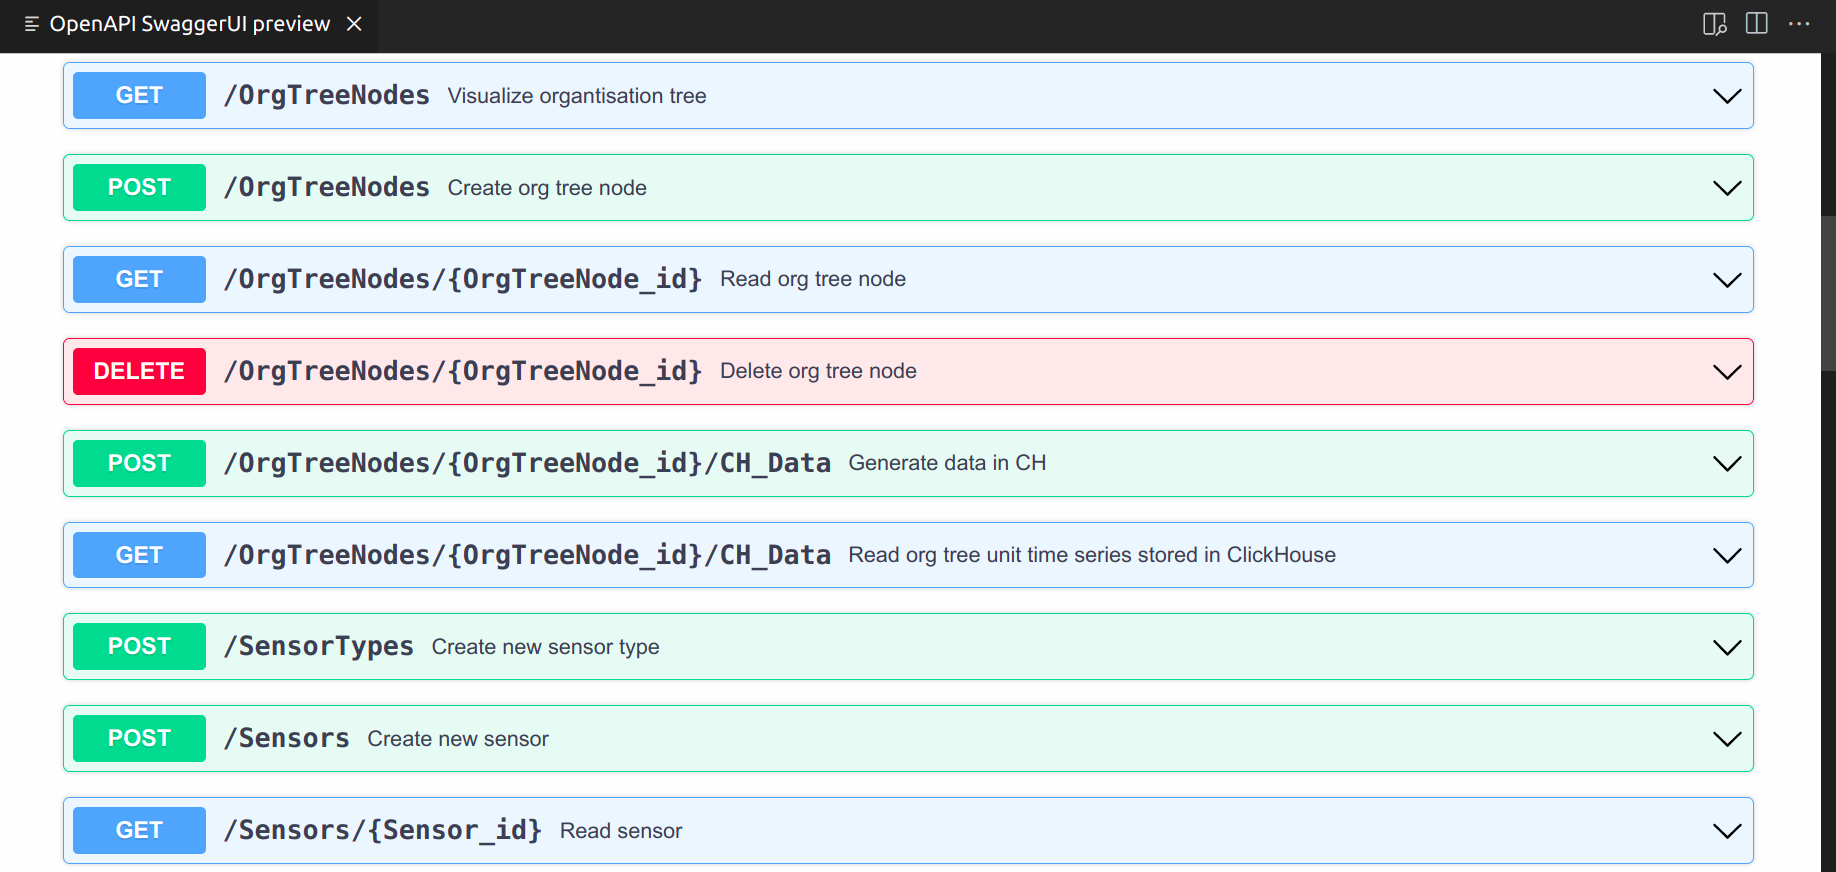
\includegraphics[scale=0.2]{img/swagger1.png}
    \caption{SwaggerUI}
    \label{swagger1}
\end{figure}

\begin{figure}
    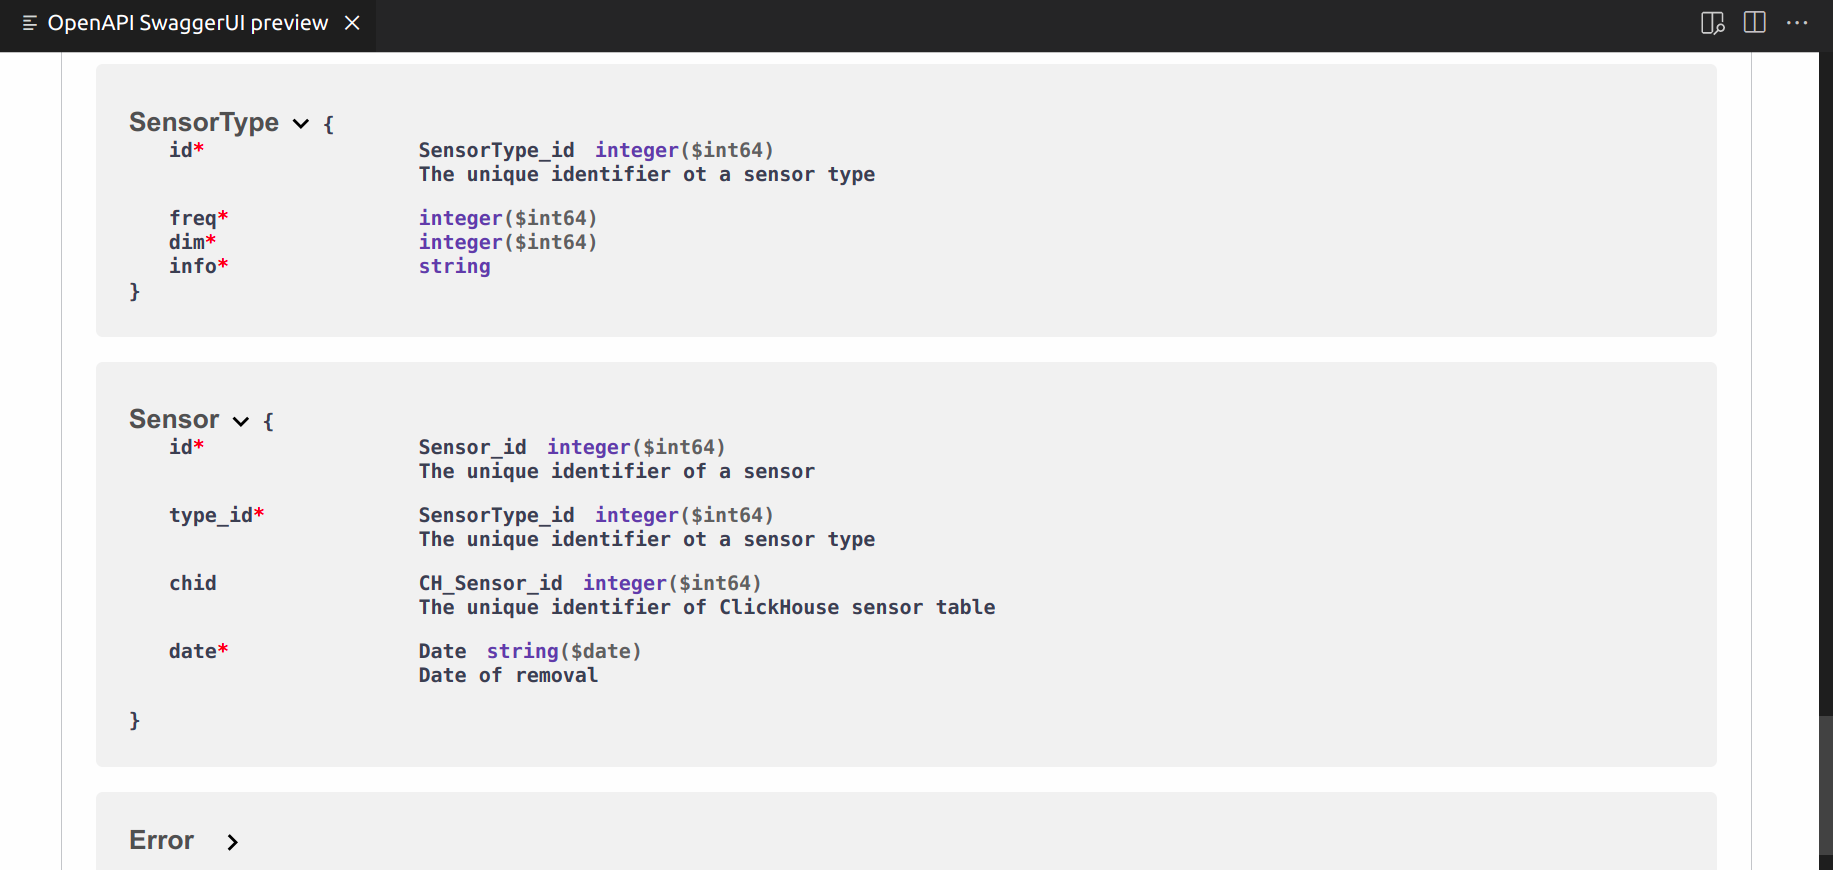
\includegraphics[scale=0.2]{img/swagger2.png}
    \caption{Справочная информация в SwaggerUI}
    \label{swagger2}
\end{figure}

Создадим новую организационную единицу <<My special org unit>>. Это можно сделать, открыв <<POST /OrgUnits>>, как показано на рисунке~\ref{swagger3}. Чтобы создать вершину дерева для этой организационной единицы, необходимо отправить POST запрос во вкладке /OrgTreeNodes как на рисунке ~\ref{swagger5}. Результаты выполнения запросов приведены на рисунках ~\ref{swagger4} и ~\ref{swagger6} соответственно.

\begin{figure}
    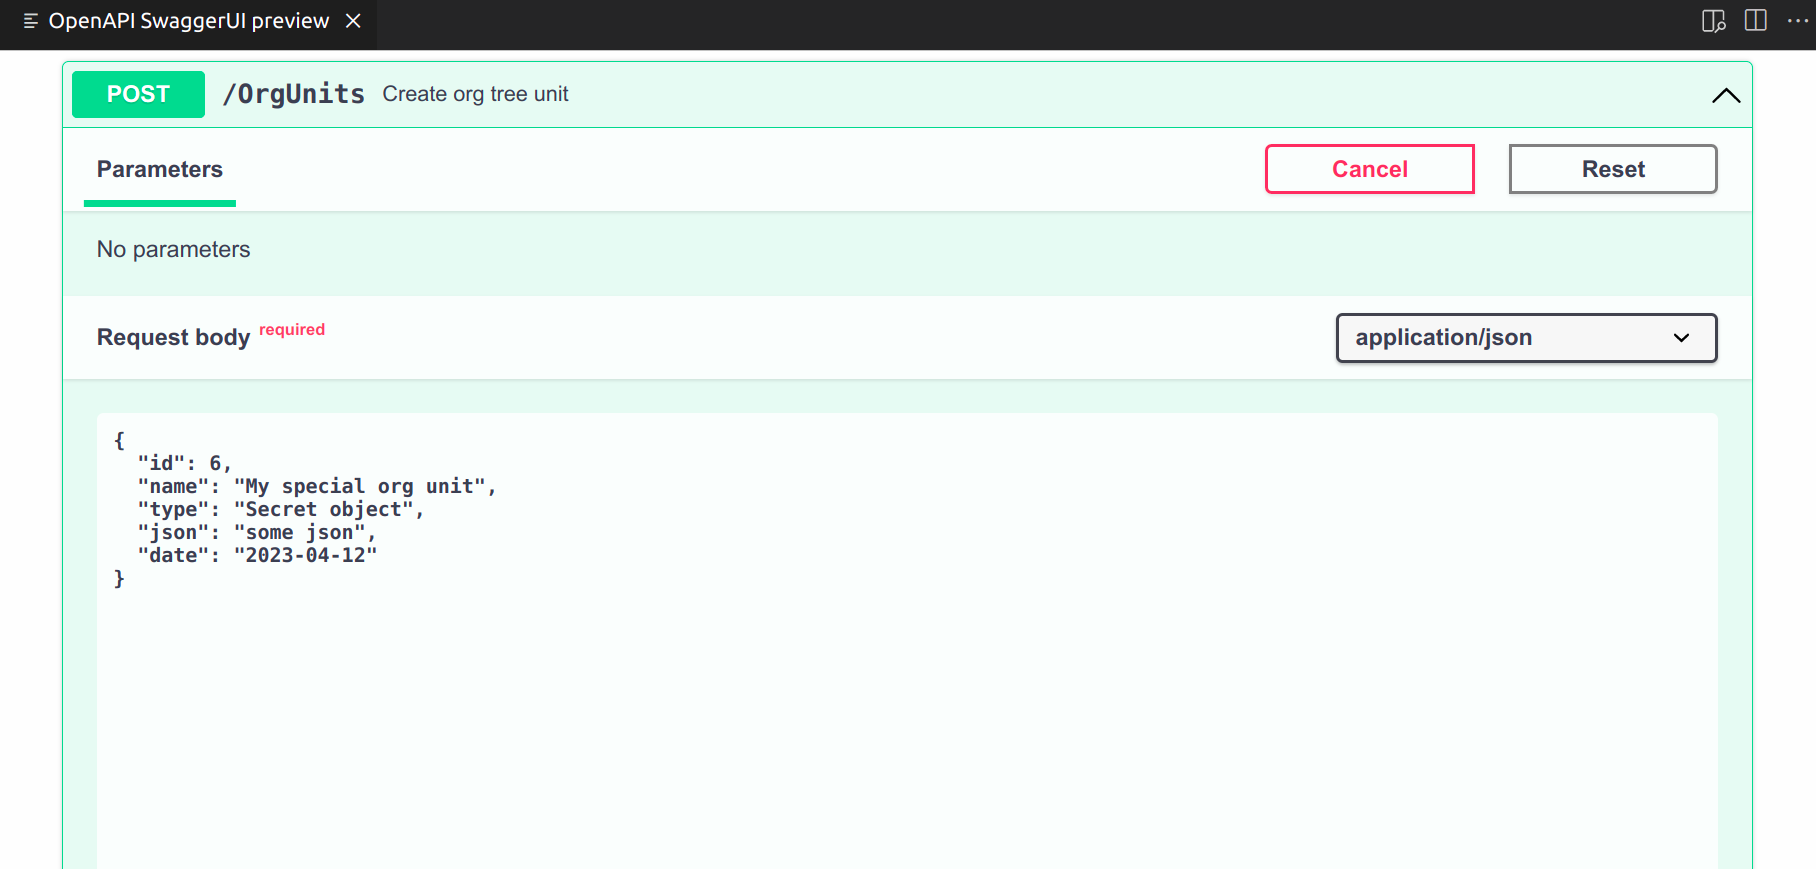
\includegraphics[scale=0.2]{img/swagger3.png}
    \caption{Добавление новой организационной единицы}
    \label{swagger3}
\end{figure}

\begin{figure}
    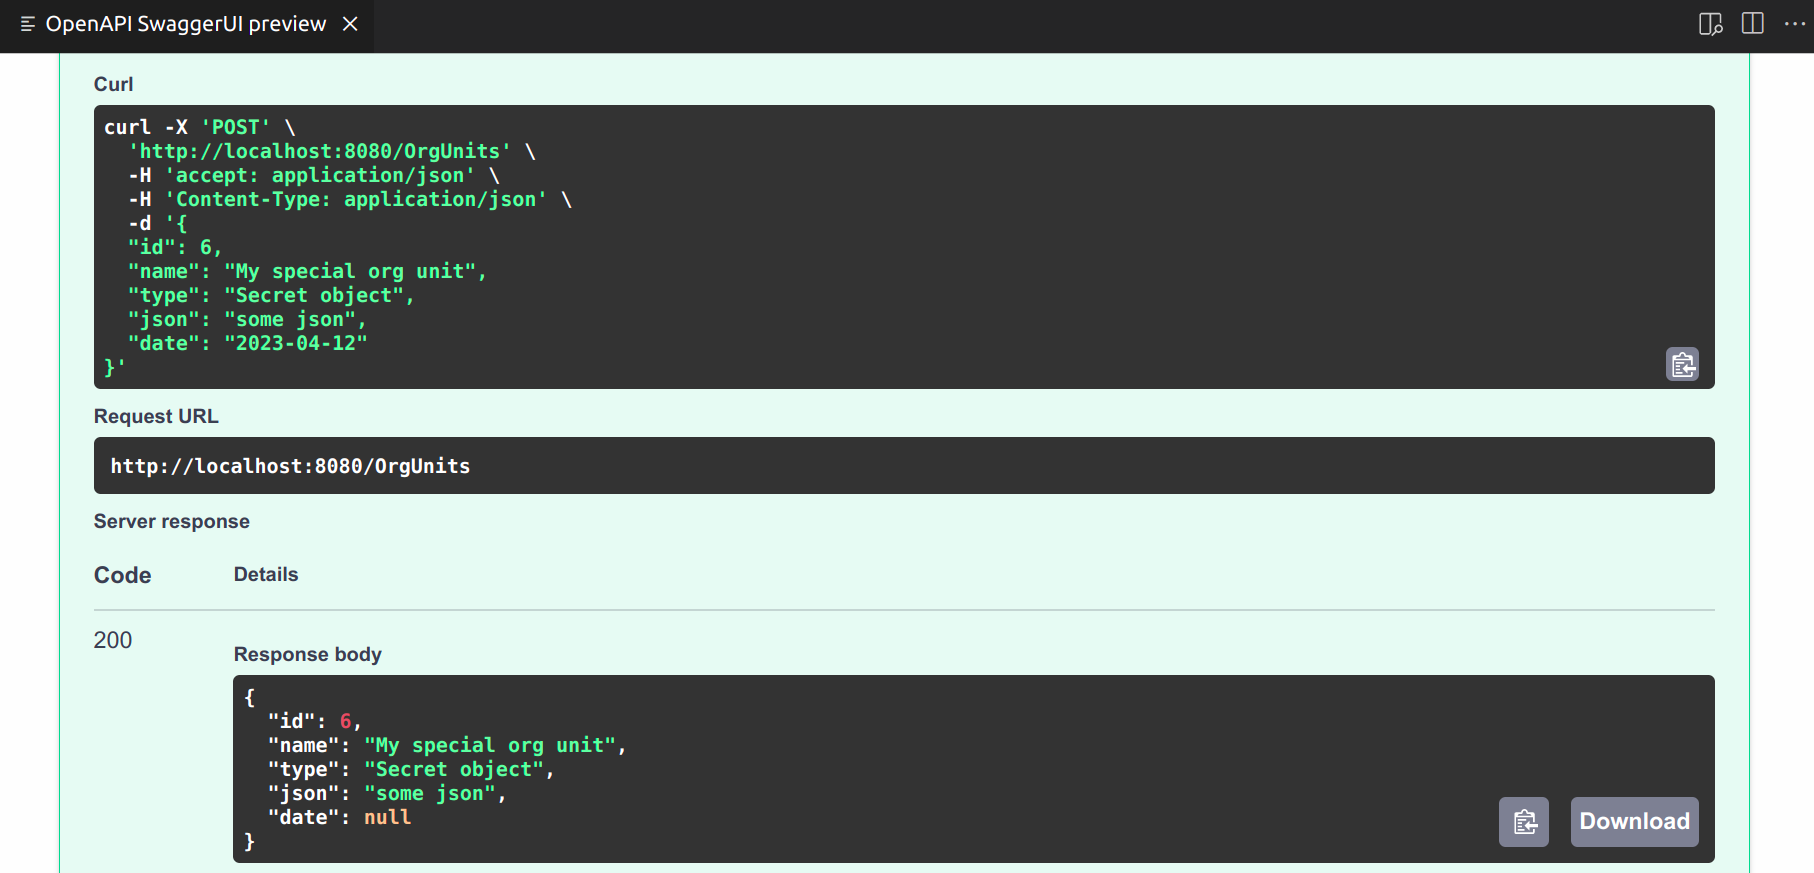
\includegraphics[scale=0.2]{img/swagger4.png}
    \caption{Ответ на запрос добавления организационной единицы}
    \label{swagger4}
\end{figure}

\begin{figure}
    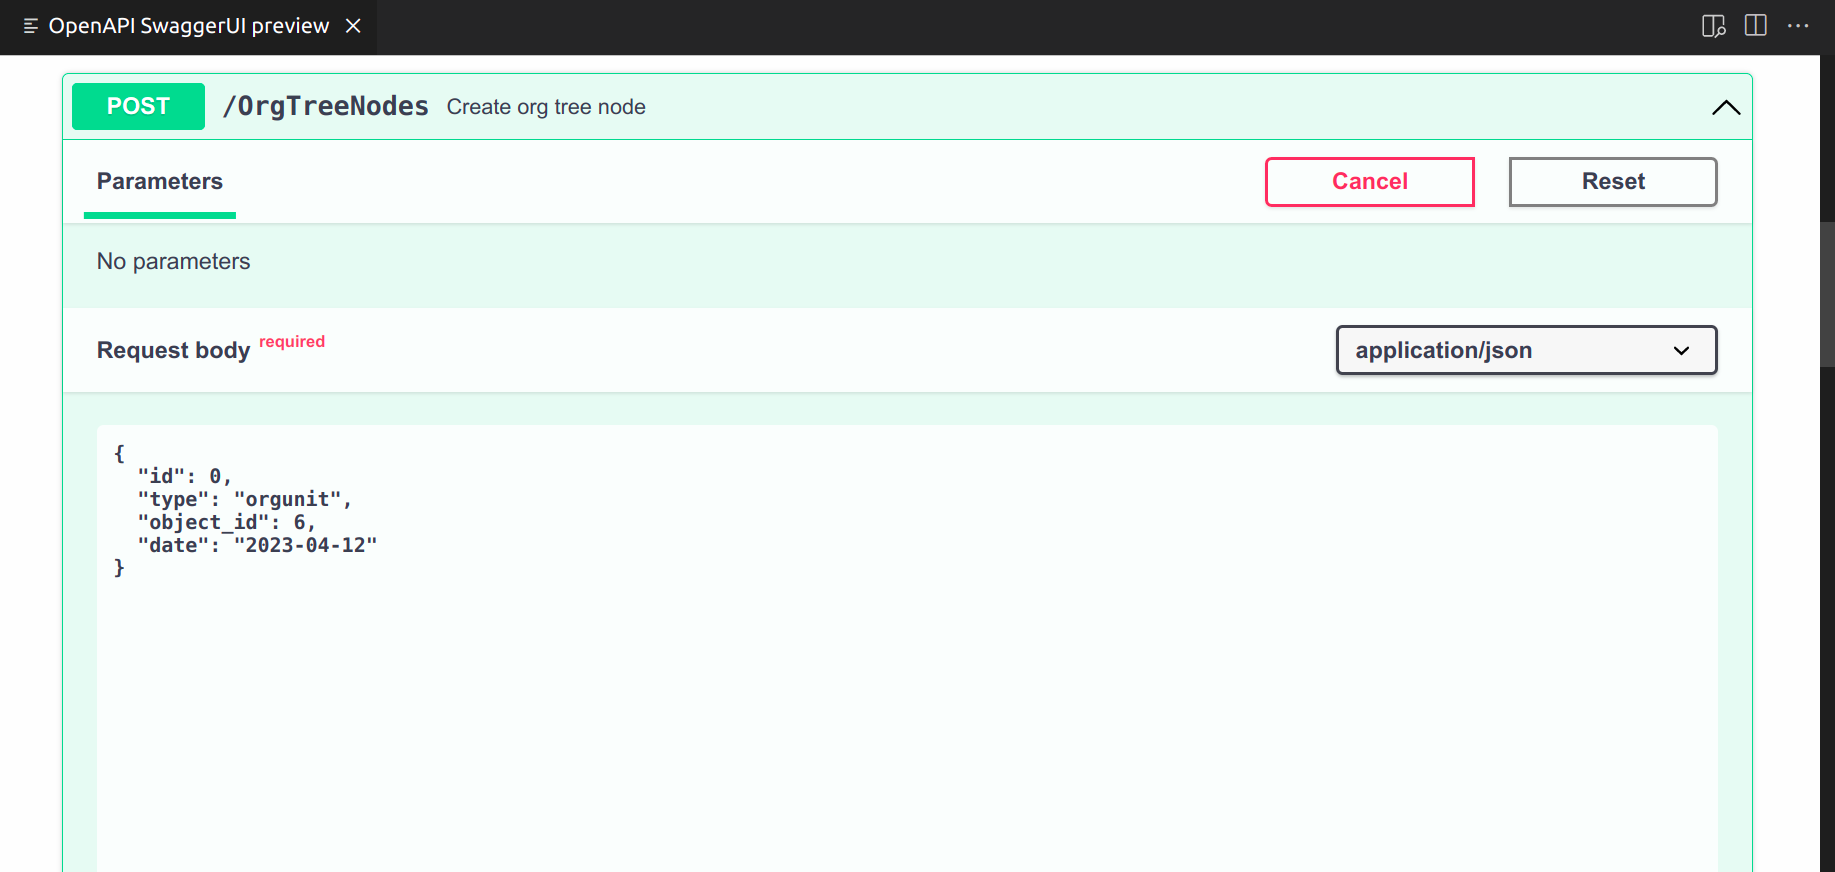
\includegraphics[scale=0.2]{img/swagger5.png}
    \caption{Добавление новой вершины дерева}
    \label{swagger5}
\end{figure}

\begin{figure}
    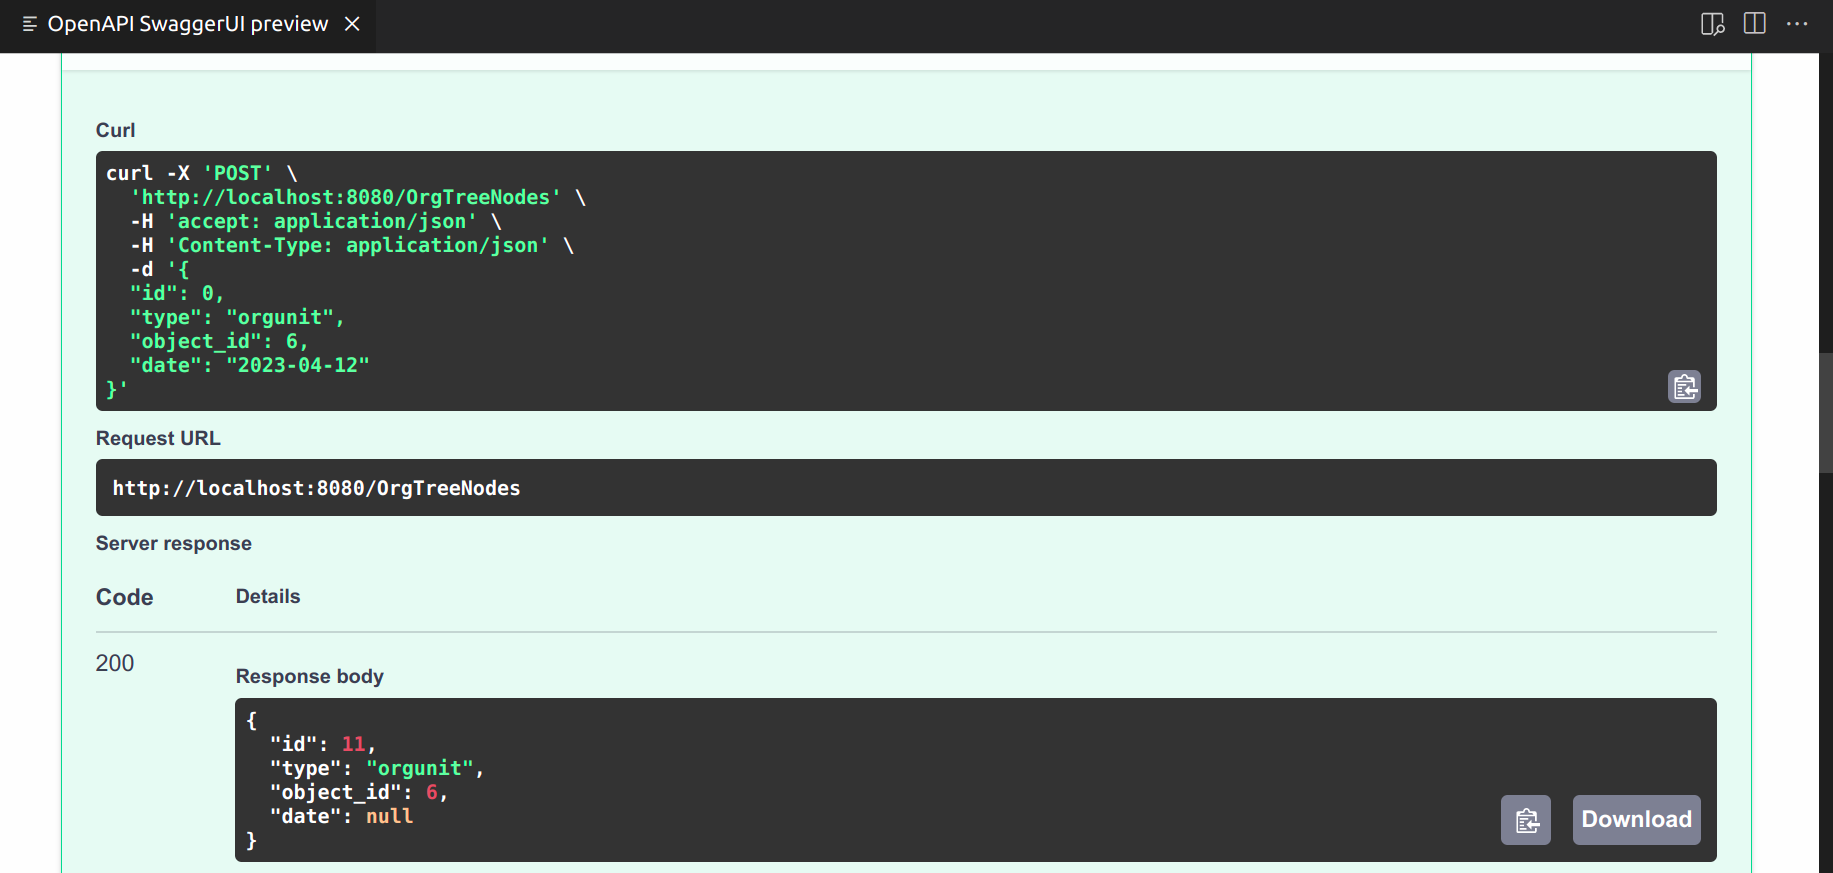
\includegraphics[scale=0.2]{img/swagger6.png}
    \caption{Ответ на запрос добавления вершины дерева}
    \label{swagger6}
\end{figure}

Вкладка /OrgTreeNodes визуализирует текущее дерево организационной структуры. Пример приведён на рисунке~\ref{demo1}. Удалённые вершины и рёбра помечаются пунктирными линиями. После удаления $8$ вершины, всё поддерево с корнем в этой вершине помечается пунктиром, что видно на рисунке~\ref{demo2}.

\begin{figure}
    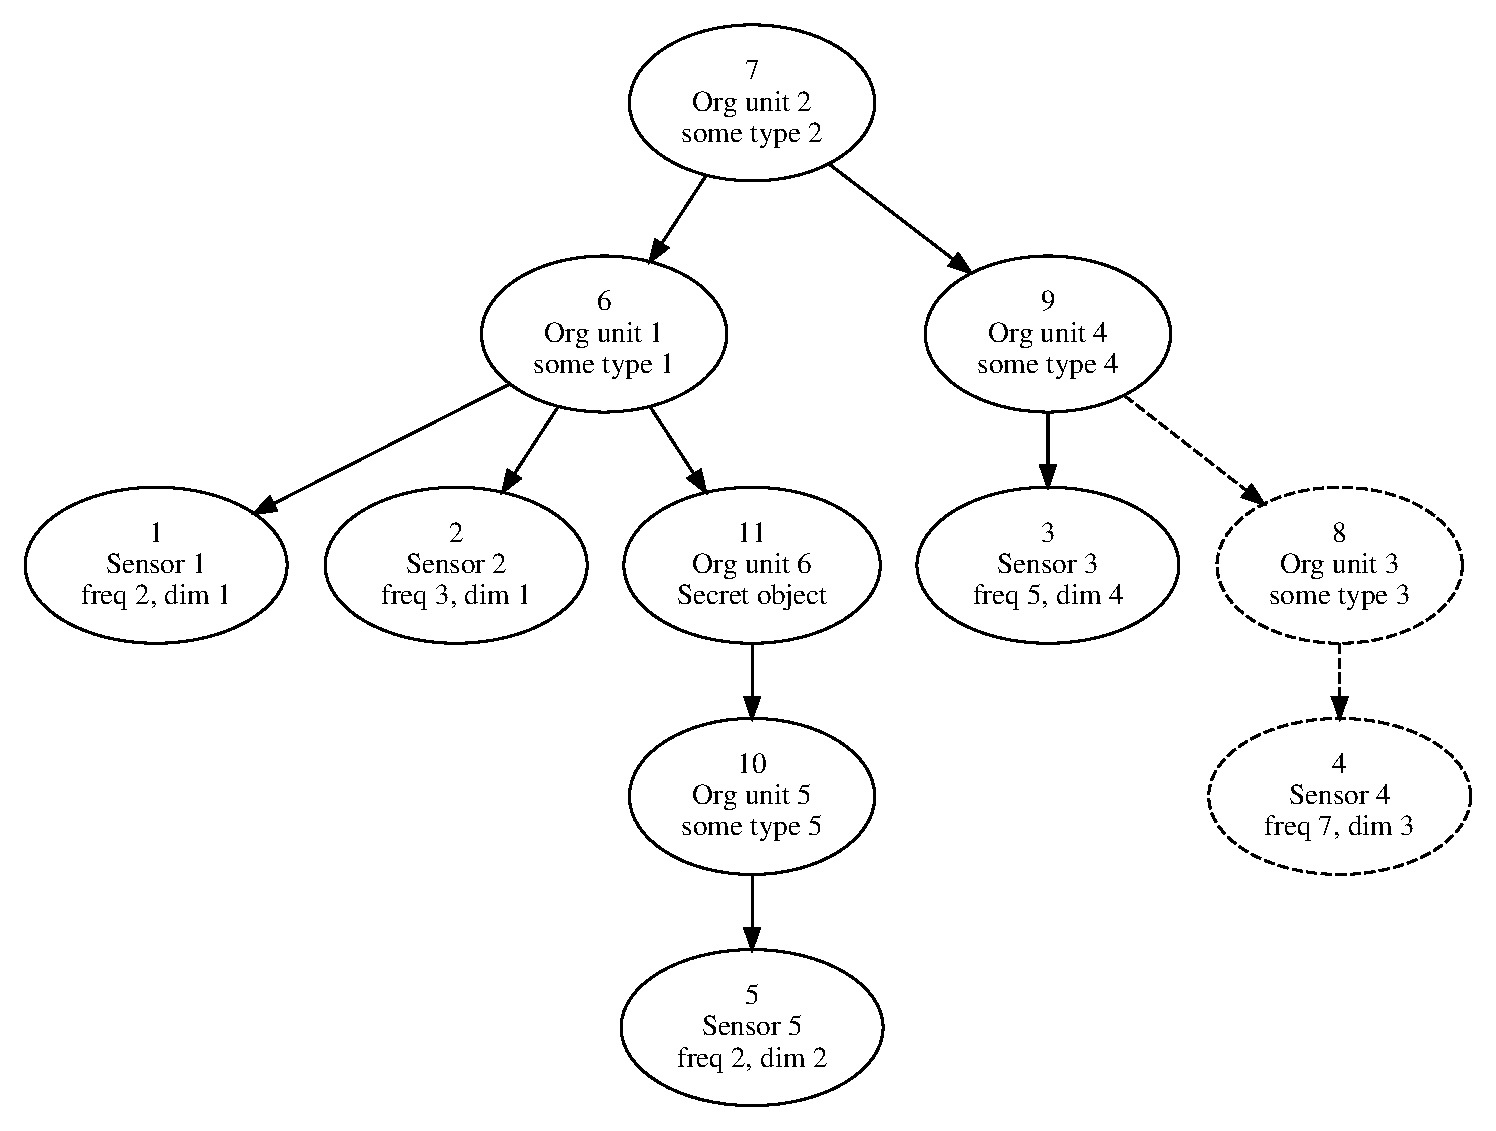
\includegraphics[scale=0.6]{img/demo_del8.eps}
    \caption{Визуализация дерева организационной структуры}
    \label{demo1}
\end{figure}

\begin{figure}
    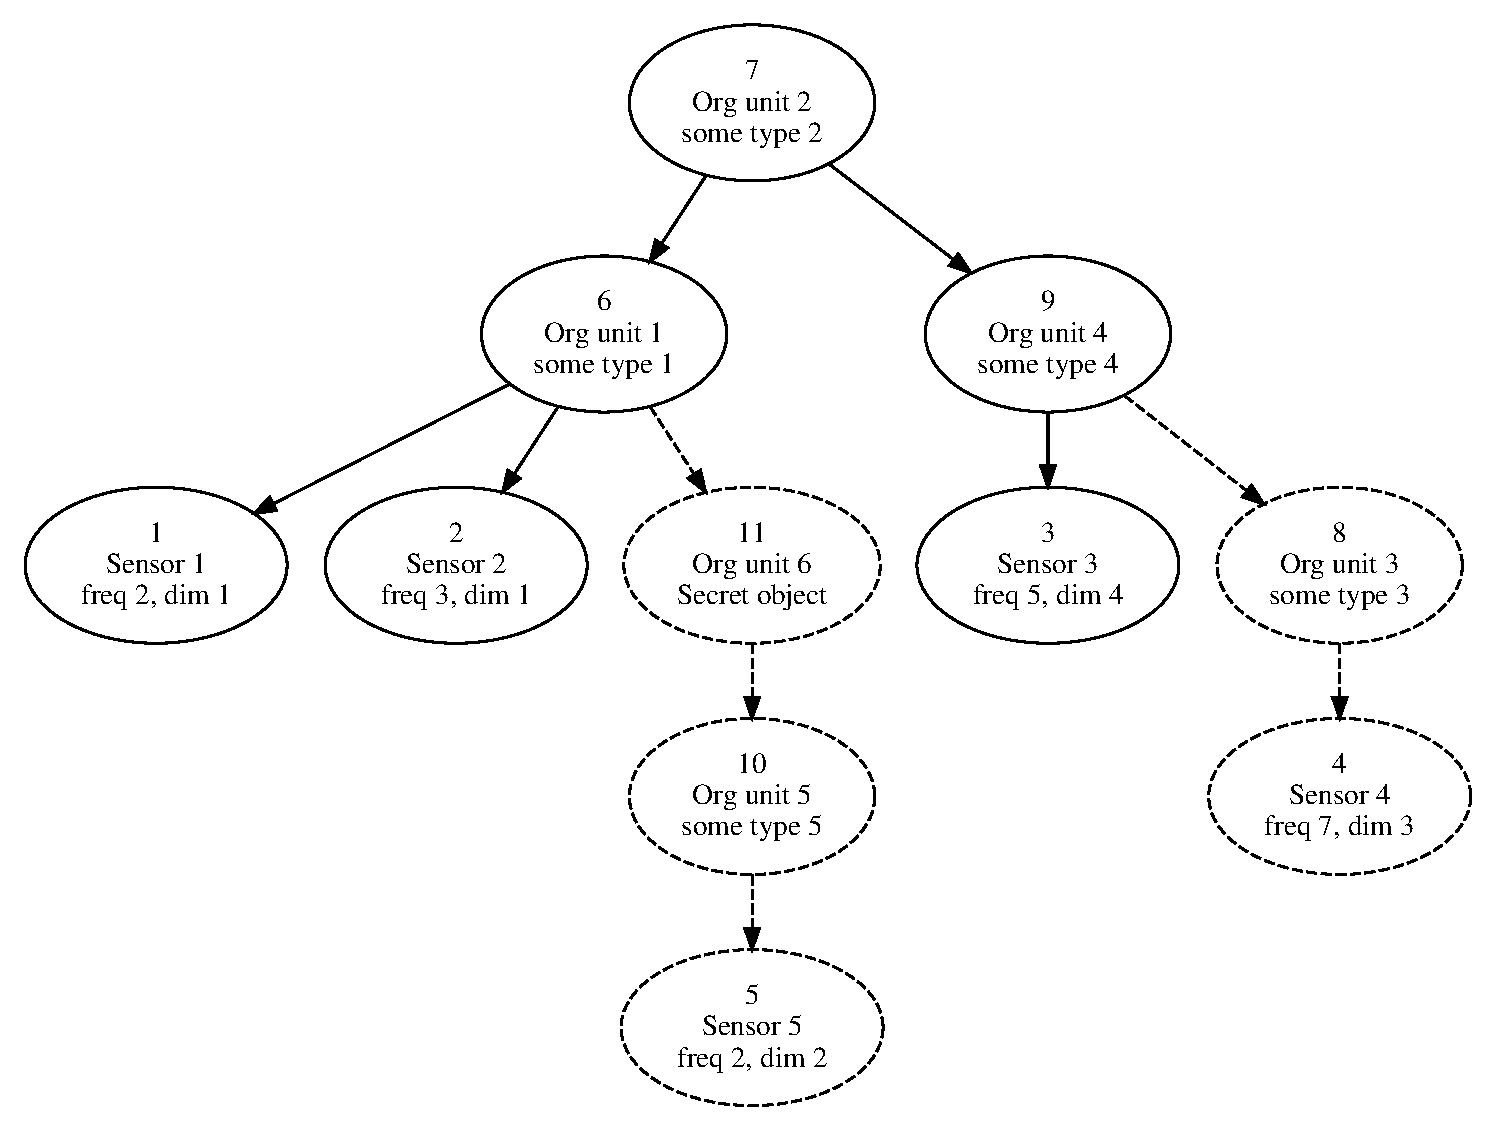
\includegraphics[scale=0.6]{img/demo_del8,11.eps}
    \caption{Визуализация дерева организационной структуры}
    \label{demo2}
\end{figure}

Для получения данных с датчиков необходимо указать номер вершины дерева и промежуток времени, что видно на рисунке~\ref{swagger7}. Результат обработки запроса изображен на рисунке~\ref{swagger8}. После удаления вершины $11$, значит и датчика $5$, данные с него не будут собраны, как показано на рисунке~\ref{swagger9}.

\begin{figure}
    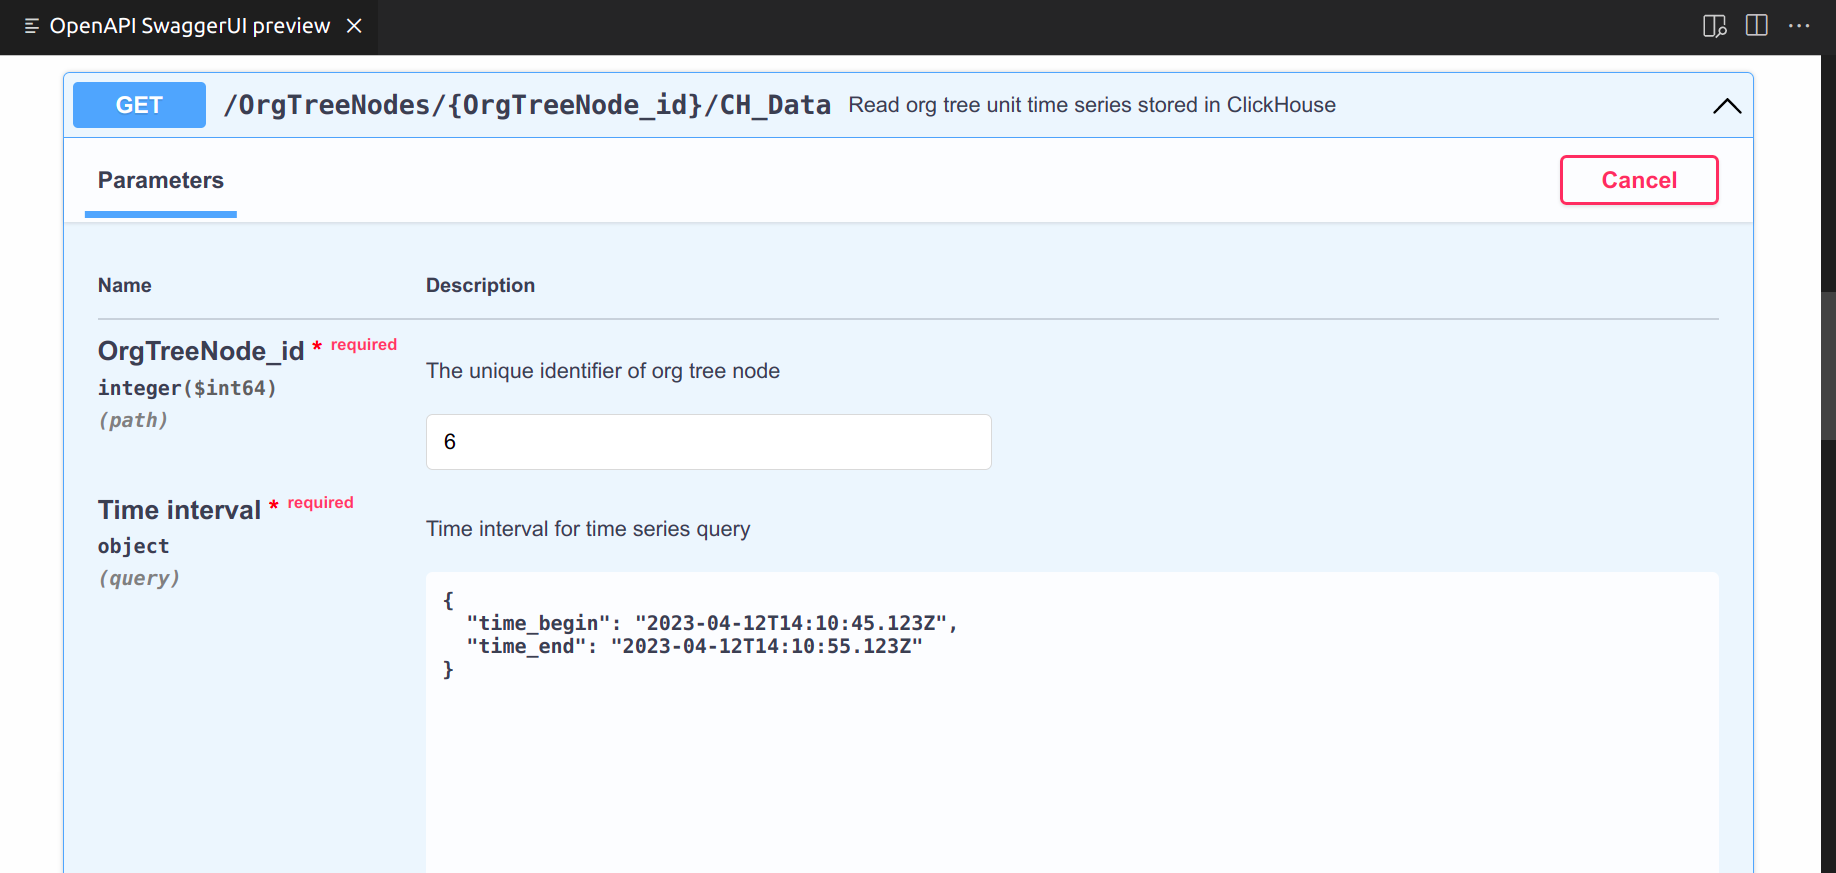
\includegraphics[scale=0.2]{img/swagger7.png}
    \caption{Запрос получения данных с датчиков}
    \label{swagger7}
\end{figure}

\begin{figure}
    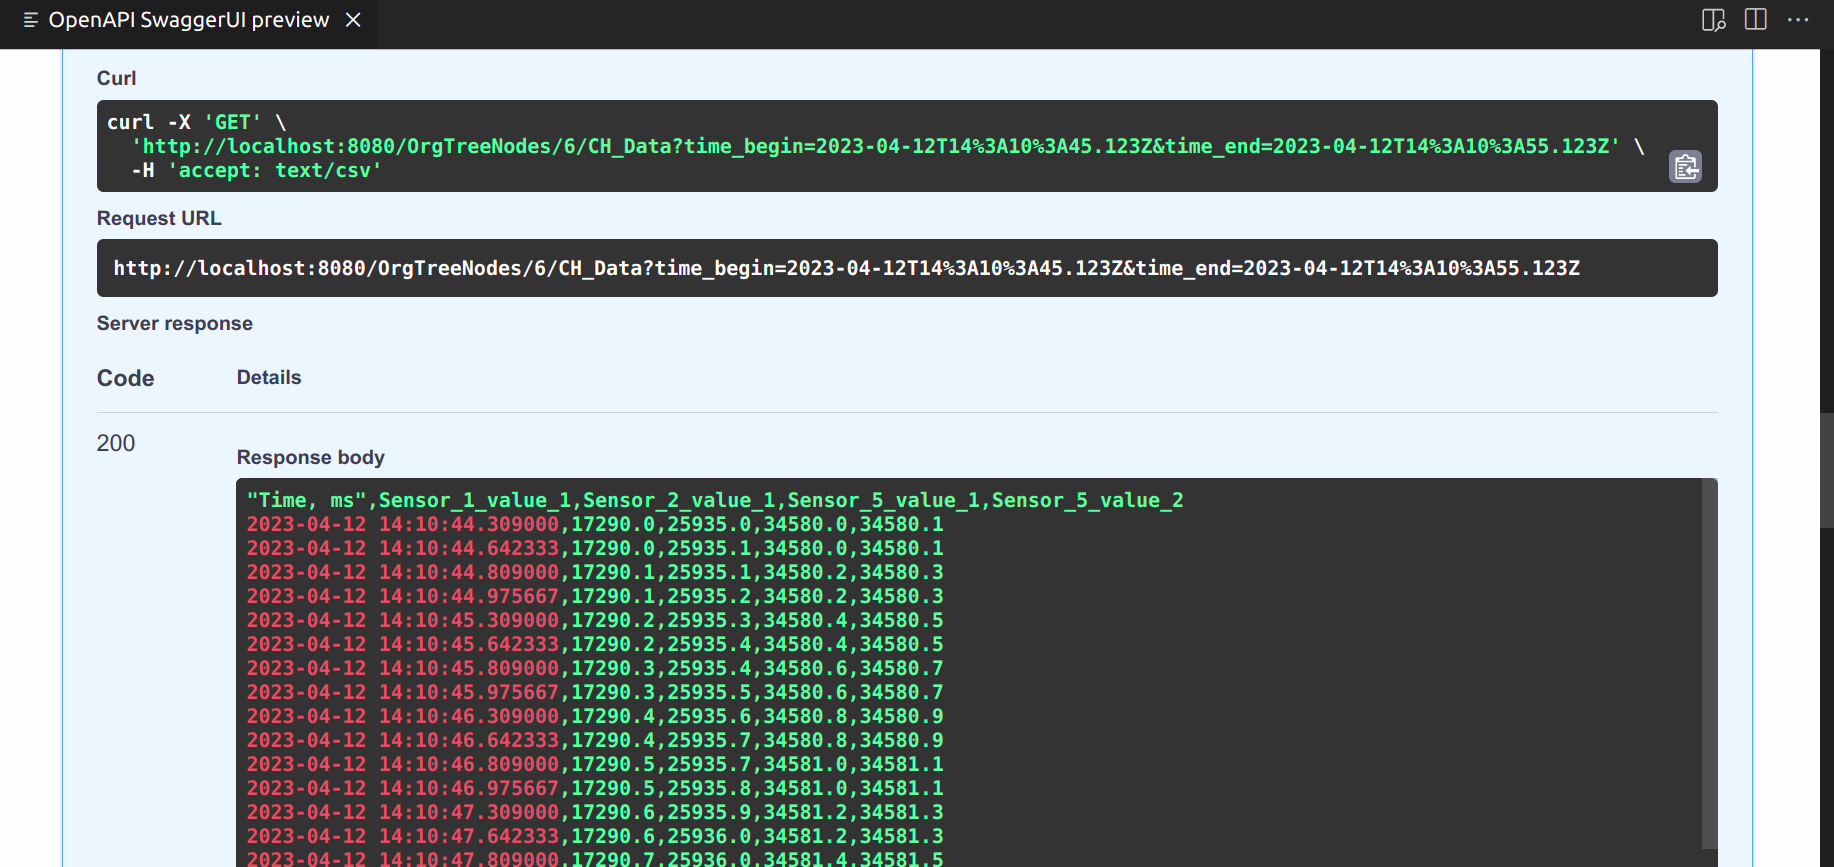
\includegraphics[scale=0.2]{img/swagger8.png}
    \caption{Временные ряды с датчиков $1$, $2$, $5$}
    \label{swagger8}
\end{figure}

\begin{figure}
    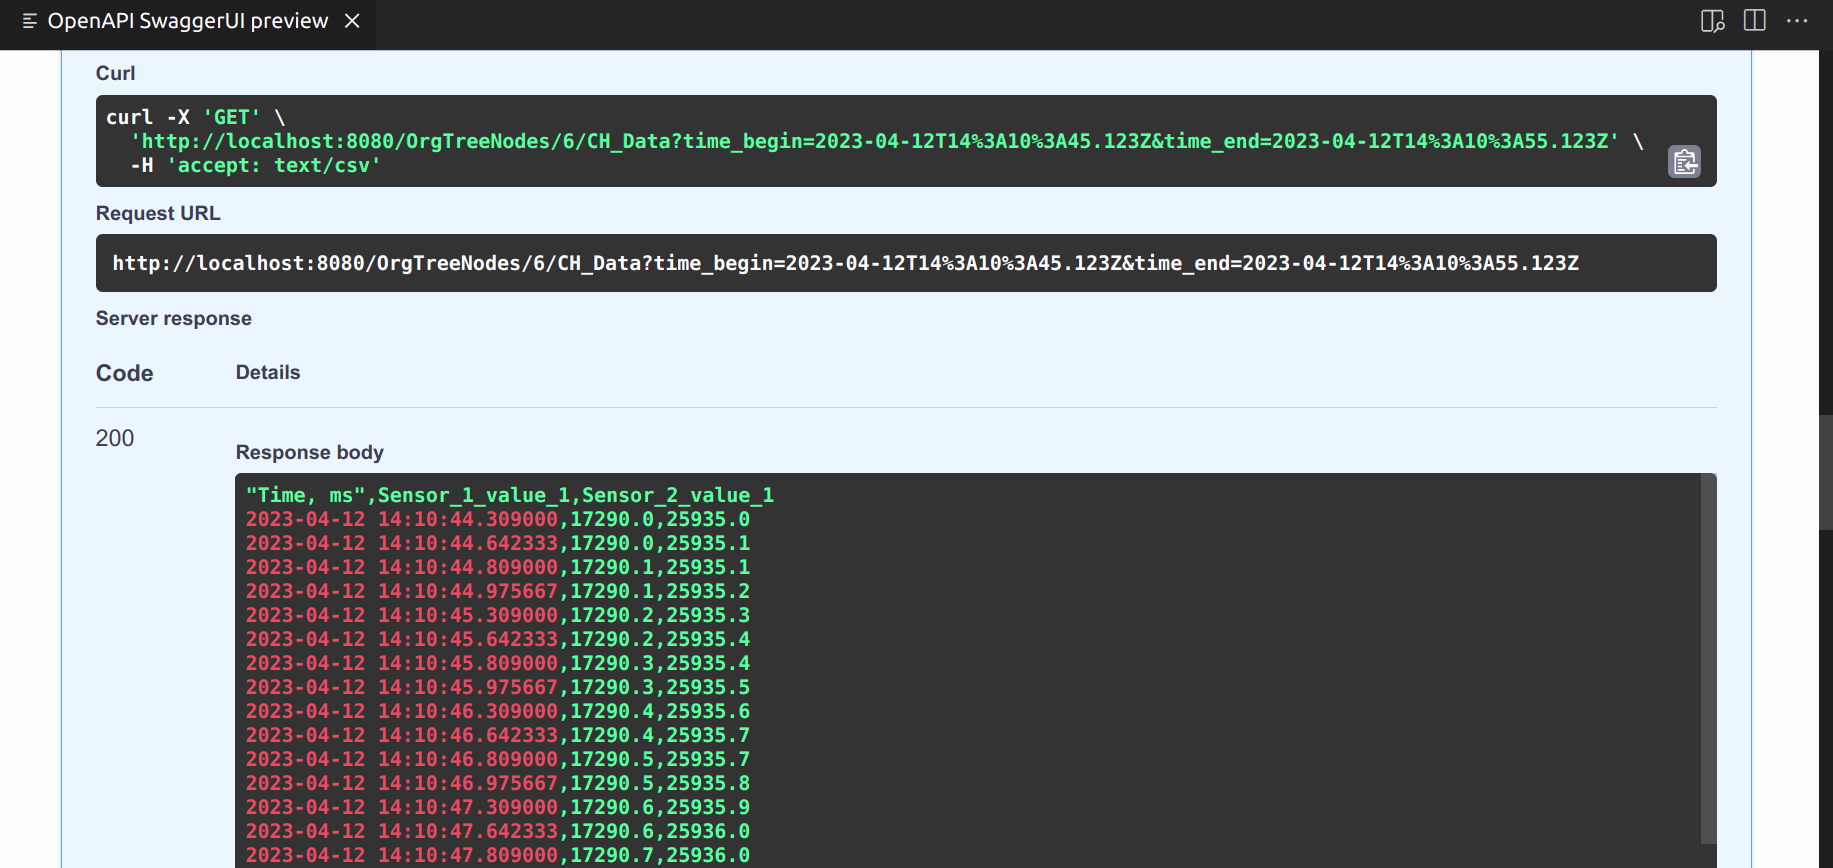
\includegraphics[scale=0.2]{img/swagger9.png}
    \caption{Временные ряды с датчиков $1$, $2$}
    \label{swagger9}
\end{figure}

Данные с датчиков сохраняются в csv таблице на диске, так как их может быть очень много. Выше полученные файлы преобразуются в JSON для наглядности.

\subsection{Тесты производительности}

Ранее был приведён алгоритм управления временными рядами, где каждому датчику соответствует отдельная таблица в ClickHouse. Другой подход --- поддерживать одну таблицу для всех датчиков, предварительно выполнив интерполяцию, и отвечать на запрос получения временных рядов, считывая нужные данные.

Для сравнения этих двух подходов в работе генерируются данные и вставляют в таблицы, затем формируются запросы на получение временных рядов датчиков на заданных временных интервалах различной длинны.

Тестирование проводилось на электронной вычислительной машине со следующими техническими характеристиками и программным обеспечением:

\begin{itemize}
    \item центральный процессор <<Intel i7-9750H (12) @ 4.500GHz>>;
    \item оперативная память: два модуля <<Kingston KHX2666C15S4/16G 16384 MB @ 2667MHz>>;
    \item твердотельный накопитель: <<KINGSTON RBUSNS8154P3256GJ (E8FK11.C) 256 GB>>;
    \item операционная система <<Ubuntu 20.04.5 LTS x86\_64>>;
    \item Python 3.8.10;
    \item Docker version 20.10.17, build 100c70180f;
    \item Docker Compose version v2.17.2.
\end{itemize}

Дерево организационной структуры, используемое при тестировании изображено на рисунке~\ref{bench-graph}. Все запросы формируются к вершины под номером $7$, соответствующей организационной единице <<Org unit $2$>>. Таким образом в тесте задействованы датчики под номера $1$, $2$, $3$, $4$ с частотами дискретизации $2$, $3$, $5$ и $7$ соответственно.

\begin{figure}
    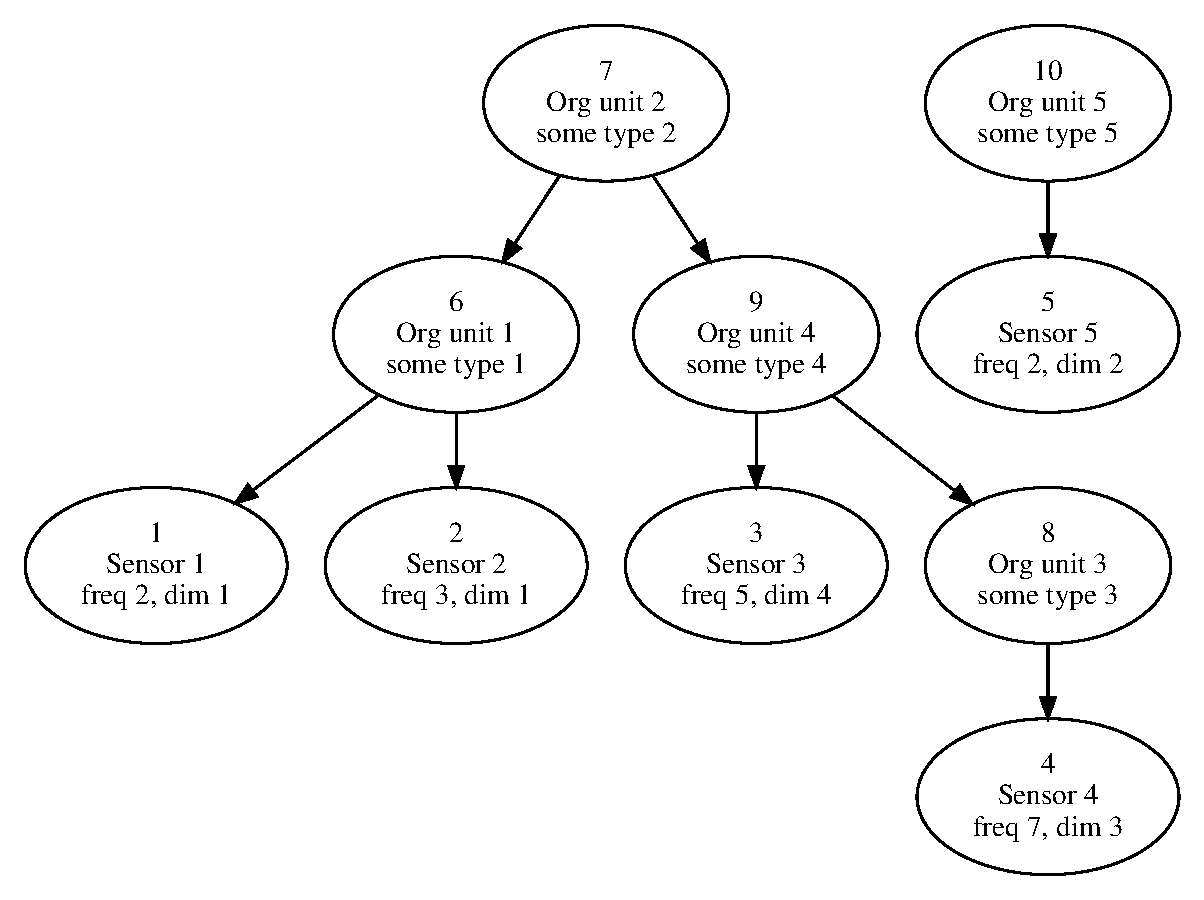
\includegraphics[scale=0.6]{img/bench.eps}
    \caption{Дерево организационной структуры в тесте производительности}
    \label{bench-graph}
\end{figure}

Данные датчиков генерируются на временном интервале $2 \cdot {10} ^ {6}$ секунд. С учётом частот опроса это вставка $3.4 \cdot {10} ^ {7}$ записей в таблицы. Вставка в разные таблицы была выполнена за $155.49$ секунд, а в одну большую таблицу за $262.83$ секунды, так как в ней сразу выполнялась интерполяции значений датчиков.

Для сравнения производительности получения временных рядов были выполнены запросы для временных интервалов длинной $100$, $200$, $500$, $1000$, $2000$, $5000$, $10000$, $20000$, $50000$, $100000$ и $200000$ секунд. Графики времени обработки запроса для длинн до $20000$ секунд приведены на рисунке~\ref{bench2e4}. Видно, что на интерполяцию значений из нескольких таблиц уходит примерно на $20\%$ больше времени.

\begin{figure}
    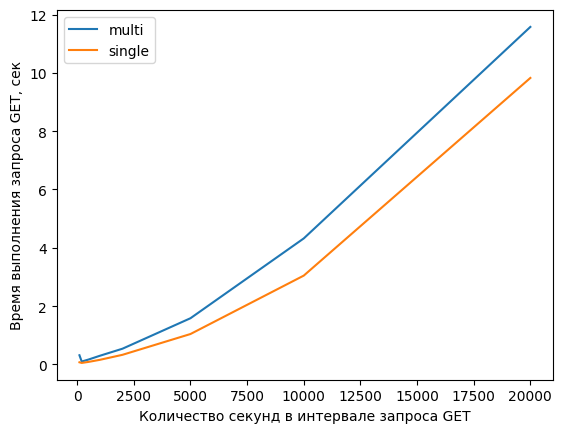
\includegraphics[scale=1.0]{img/bench2e4.png}
    \caption{Графики времени обработки маленьких запросов}
    \label{bench2e4}
\end{figure}

Графики времени обработки запросов для больших временных инервалов приведены на рисунке~\ref{bench2e5}. Интерполяция значений из нескольких таблиц обгоняет и существенно опережает получение данных из одной таблицы. Так как таблицы баз данных хранятся на постоянном запоминающем устройстве компьютера, считывание информации из них занимает больше времени, чем интерполяция в оперативной памяти компьютера. На маленьких временных интервалах затраты на объединение таблиц выше, чем на считывание, однако на больших запросов результат противоположный.

\begin{figure}
    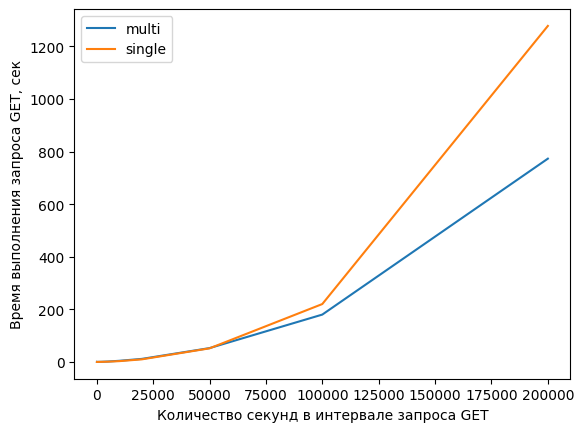
\includegraphics[scale=1.0]{img/bench2e5.png}
    \caption{Графики времени обработки больших запросов}
    \label{bench2e5}
\end{figure}

Из теста производительности следует, что вариант с таблицей под каждый датчик выигрывает по времени у варианта с одной таблицей. Получение временного ряда длительностью $200000$ секунд, что составляет около $3.4 \cdot {10} ^ {6}$ строк в итоговой матрице, заняло $773.06$ секунд.

ClickHouse способен обрабатывать порядка ${10} ^ {6}$ строк в секунду, поэтому для улучшения производительности программы можно сравнить разные алгоритмы сортировок. Python упрощает разработку динамической типизацией, однако это замедляет программу. Решения на C и C++ обычно быстрее тех, что реализованы на Python, на один-два порядка. При необходимости увеличения производительности время обработки больших запросов может быть сокращено с десяти до пары минут.
 % Глава 3

\conclusion

В результате выполнения выпускной квалификационной работы бакалавра был разработан модуль управления временными рядами сигналов сложных технических систем на языке Python с использованием СУБД PostgreSQL и ClickHouse. Были решены следующие задачи:

\begin{itemize}
    \item спроектирована модель данных дерева организационной структуры предприятия;
    \item описаны способы взаимодействия: добавление, удаление и изменение вершин и рёбер дерева;
    \item спроектирована модель хранения временных рядов датчиков;
    \item изучены средства и технологии, которые будут применятся в ходе разработки программного продукта;
    \item реализован модуль управления графом организационной структурой и данными;
    \item разработан алгоритм объединения данных датчиков с разными частотами дискретизации;
    \item реализована генерация данных для таблиц датчиков, алгоритм получения наборов временных рядов;
    \item произведён тест производительности реализованного модуля, проведено сравнение двух алгоритмов хранения и считывания данных.
\end{itemize}

Базы данных хранятся в постоянной памяти компьютера. Твердотельные накопители быстрее записывают и считывают данные, что может ускорить работу модуля. Для повышения надёжности рекомендуется создавать резервные копии баз данных, сохраняя их на жёсткий диск.

Созданный модуль позволяет изменить структуру дерева организационной структуры на предприятии, добавлять и удалять новые организационные единицы и датчики, изменять их параметры. Удалённые объекты хранятся в базе данных, чтобы была возможность сформировать список изменений.

При получении набора временных рядов датчиков с разными частотами дискретизации неизвестные значения интерполируются по последним известным.

Модуль автоматизирует сбор информации с сенсоров системы, тем самым упрощая создание цифрового двойника электростанции. Данные с датчиков надёжно хранятся в базе данных и будут использованы для моделирования объекта и предиктивной аналитики. Так можно будет оптимизировать работу оборудования, уменьшая скорость износа и повышая отказоустойчивость как отдельной электростанции, так и всей электросети в целом.
 % Заключение

\printbibliography % Список литературы

\appendix % Приложения
\appendixsection{Исходный код}

На рисунке~\ref{qr} изображен QR-код со ссылкой на GitHub репозиторий с исходным кодом разработанного программного продукта.

\begin{figure}
    
\includegraphics[width=5cm]{../img/qr-git.eps}
    \caption{QR-код на репозиторий}
    \label{qr}
\end{figure}

\end{document}
